%%%%%%%%%%%%%%%%%%%%%%%%%%%%%%%%%%%%%%%%%
% Masters/Doctoral Thesis
% LaTeX Template
% Version 2.5 (27/8/17)
%
% This template was downloaded from:
% http://www.LaTeXTemplates.com
%
% Version 2.x major modifications by:
% Vel (vel@latextemplates.com)
%
% This template is based on a template by:
% Steve Gunn (http://users.ecs.soton.ac.uk/srg/softwaretools/document/templates/)
% Sunil Patel (http://www.sunilpatel.co.uk/thesis-template/)
%
% Template license:
% CC BY-NC-SA 3.0 (http://creativecommons.org/licenses/by-nc-sa/3.0/)
%
%%%%%%%%%%%%%%%%%%%%%%%%%%%%%%%%%%%%%%%%%

%----------------------------------------------------------------------------------------
%	PACKAGES AND OTHER DOCUMENT CONFIGURATIONS
%----------------------------------------------------------------------------------------

\documentclass[
11pt, % The default document font size, options: 10pt, 11pt, 12pt
oneside, % Two side (alternating margins) for binding by default, uncomment to switch to one side
spanish, % ngerman for German
singlespacing, % Single line spacing, alternatives: onehalfspacing or doublespacing
%draft, % Uncomment to enable draft mode (no pictures, no links, overfull hboxes indicated)
%nolistspacing, % If the document is onehalfspacing or doublespacing, uncomment this to set spacing in lists to single
%liststotoc, % Uncomment to add the list of figures/tables/etc to the table of contents
%toctotoc, % Uncomment to add the main table of contents to the table of contents
%parskip, % Uncomment to add space between paragraphs
%nohyperref, % Uncomment to not load the hyperref package
headsepline, % Uncomment to get a line under the header
%chapterinoneline, % Uncomment to place the chapter title next to the number on one line
%consistentlayout, % Uncomment to change the layout of the declaration, abstract and acknowledgements pages to match the default layout
]{MastersDoctoralThesis} % The class file specifying the document structure

\usepackage[utf8]{inputenc} % Required for inputting international characters
\usepackage[T1]{fontenc} % Output font encoding for international characters

\usepackage[fleqn]{amsmath}
\usepackage{amssymb}
\usepackage{amsthm}
\usepackage{stmaryrd}
\SetSymbolFont{stmry}{bold}{U}{stmry}{m}{n}
\usepackage{physics}
\usepackage{proof}
\usepackage{todonotes}

\usepackage[backend=biber,style=nature,sorting=nty]{biblatex}

\newtheorem{theorem}{Teorema}[chapter]
\newtheorem{lemma}[theorem]{Lema}
\newtheorem{conjecture}[theorem]{Conjetura}
\theoremstyle{definition}
\newtheorem{definition}[theorem]{Definición}

\addbibresource{bibliography.bib} % The filename of the bibliography

\usepackage[autostyle=true]{csquotes} % Required to generate language-dependent quotes in the bibliography

\newcommand{\qubittype}{\mathbb{B}}
\newcommand{\snset}{\mathsf{FN}}
\newcommand{\neutralset}{\mathcal{N}}
\newcommand{\interp}[1]{\llbracket#1\rrbracket}
\newcommand{\vrbl}[2]{#1^{#2}}
\newcommand{\nullvec}[1]{\vec{0}_{S (#1)}}
\newcommand{\ifte}[3]{#1? #2 \cdot #3}
\newcommand{\red}[1]{\mathsf{Red} (#1)}
\newcommand{\head}[1]{\mathsf{head}~#1}
\newcommand{\tail}[2][]{\mathsf{tail}^{#1}~#2}
\newcommand{\cast}[2]{\Uparrow_{#1}^{#2}}
\newcommand{\proj}[2]{\pi_{#1} #2}
\newcommand{\lpl}[1]{|#1|}
\newcommand{\size}[1]{||#1||}
\newcommand{\reducesto}{\rightarrow}
\newcommand{\abstr}[2]{\lambda#1\ldotp#2}
\newcommand{\lcabstr}[2]{(\lambda#1\ldotp#2)}
\newcommand{\stlcabstr}[3]{(\lambda#1^#2\ldotp#3)}
\newcommand{\app}[2]{#1 #2}
\newcommand{\lcapp}[2]{(#1 #2)}
\newcommand{\stlcapp}[2]{(#1 #2)}
\newcommand{\lambdacalculus}{\lambda\text{-cálculo}}
\newcommand{\lambdas}{\lambda_S}
\newcommand{\tensor}{\otimes}

%----------------------------------------------------------------------------------------
%	MARGIN SETTINGS
%----------------------------------------------------------------------------------------

\geometry{
	paper=a4paper, % Change to letterpaper for US letter
	inner=2.5cm, % Inner margin
	outer=3.8cm, % Outer margin
	bindingoffset=.5cm, % Binding offset
	top=1.5cm, % Top margin
	bottom=1.5cm, % Bottom margin
	%showframe, % Uncomment to show how the type block is set on the page
}

%----------------------------------------------------------------------------------------
%	THESIS INFORMATION
%----------------------------------------------------------------------------------------

\thesistitle{Demostrando normalización fuerte sobre una extensión cuántica del lambda cálculo} % Your thesis title, this is used in the title and abstract, print it elsewhere with \ttitle
\supervisor{Dr.\ Alejandro \textsc{Díaz-Caro}} % Your supervisor's name, this is used in the title page, print it elsewhere with \supname
\examiner{} % Your examiner's name, this is not currently used anywhere in the template, print it elsewhere with \examname
\degree{Licenciado en Ciencias de la Computación} % Your degree name, this is used in the title page and abstract, print it elsewhere with \degreename
\author{Juan Pablo \textsc{Rinaldi}} % Your name, this is used in the title page and abstract, print it elsewhere with \authorname
\addresses{} % Your address, this is not currently used anywhere in the template, print it elsewhere with \addressname

\subject{Ciencias de la Computación} % Your subject area, this is not currently used anywhere in the template, print it elsewhere with \subjectname
\keywords{} % Keywords for your thesis, this is not currently used anywhere in the template, print it elsewhere with \keywordnames
\university{\href{https://www.unr.edu.ar/}{Universidad Nacional de Rosario}} % Your university's name and URL, this is used in the title page and abstract, print it elsewhere with \univname
\department{\href{https://dcc.fceia.unr.edu.ar/}{Departamento de Ciencias de la Computación}} % Your department's name and URL, this is used in the title page and abstract, print it elsewhere with \deptname
\group{\href{http://researchgroup.university.com}{Research Group Name}} % Your research group's name and URL, this is used in the title page, print it elsewhere with \groupname
\faculty{\href{http://faculty.university.com}{Facultad de Ciencias Exactas, Ingeniería y Agrimensura}} % Your faculty's name and URL, this is used in the title page and abstract, print it elsewhere with \facname

\AtBeginDocument{
\hypersetup{pdftitle=\ttitle} % Set the PDF's title to your title
\hypersetup{pdfauthor=\authorname} % Set the PDF's author to your name
\hypersetup{pdfkeywords=\keywordnames} % Set the PDF's keywords to your keywords
}

\begin{document}

\frontmatter % Use roman page numbering style (i, ii, iii, iv...) for the pre-content pages

\pagestyle{plain} % Default to the plain heading style until the thesis style is called for the body content

%----------------------------------------------------------------------------------------
%	TITLE PAGE
%----------------------------------------------------------------------------------------

\begin{titlepage}
\begin{center}

\vspace*{.06\textheight}
{\scshape\LARGE \univname\par}\vspace{1.5cm} % University name
\textsc{\Large Tesina de Licenciatura}\\[0.5cm] % Thesis type

\HRule{} \\[0.4cm] % Horizontal line
{\huge \bfseries \ttitle\par}\vspace{0.4cm} % Thesis title
\HRule{} \\[1.5cm] % Horizontal line

\begin{minipage}[t]{0.4\textwidth}
\begin{flushleft} \large
\emph{Autor:}\\
\href{https://www.linkedin.com/in/juampi}{\authorname} % Author name - remove the \href bracket to remove the link
\end{flushleft}
\end{minipage}
\begin{minipage}[t]{0.4\textwidth}
\begin{flushright} \large
\emph{Director:} \\
\href{http://diaz-caro.web.unq.edu.ar/}{\supname} % Supervisor name - remove the \href bracket to remove the link
\end{flushright}
\end{minipage}\\[3cm]

\vfill

\large \textit{Una tesina enviada en cumplimiento de los requerimientos\\ para el título de \degreename}\\[0.3cm] % University requirement text
\textit{en el}\\[0.4cm]
\deptname{}\\[2cm] % Research group name and department name

\vfill

{\large \the\year}\\[4cm] % Date
%\includegraphics{Logo} % University/department logo - uncomment to place it

\vfill
\end{center}
\end{titlepage}

%----------------------------------------------------------------------------------------
%	ABSTRACT PAGE
%----------------------------------------------------------------------------------------

\begin{abstract}
\addchaptertocentry{\abstractname} % Add the abstract to the table of contents
Una de las propiedades fundamentales de la mecánica cuántica es la del no-clonado, la cual indica que es imposible crear una copia idéntica de un estado cuántico desconocido. Los lenguajes funcionales cuánticos pueden diferenciarse dependiendo de cómo se trate dicha propiedad. Por un lado tenemos la familia de lenguajes que utilizan lógica lineal (lenguajes LL) para excluir los términos
que duplican estados. Por otro lado tenemos la familia de
lenguajes que utilizan propiedades del álgebra lineal (lenguajes AL), los cuales
admiten términos que los otros excluyen, pero los interpretan de forma diferente, evitando también el clonado.

Los lenguajes AL, al utilizar un sistema de tipos clásicos, son más sencillos que los LL, pero los primeros tienen una desventaja frente a los últimos: no soportan
fácilmente el operador de medición, elemento fundamental de la mecánica cuántica. Por este motivo se propuso desarrollar un lenguaje, \( \lambda_S \), que posea lo mejor de ambos enfoques: la elegancia de la linealidad algebraica y el soporte para el
operador de medición usando lógica lineal.

El objetivo de la presente tesina es
probar la propiedad de \textit{normalización fuerte} sobre dicho lenguaje. Esta propiedad implica que no habrá loops infinitos, y por lo tanto, un programa bien tipado no tiene ejecuciones infinitas.
\end{abstract}

%----------------------------------------------------------------------------------------
%	ACKNOWLEDGEMENTS
%----------------------------------------------------------------------------------------

\begin{acknowledgements}
%\addchaptertocentry{\acknowledgementname} % Add the acknowledgements to the table of contents
A mamá, papá y Ceci, por estar a mi lado en cada paso y brindarme su apoyo incondicional. A mi director, Jano, por tener la paciencia y disposición que pocas personas poseen. A los que se tomaron el tiempo de revisar en detalle este trabajo, especialmente Guido. Y a todas aquellas personas que de una forma u otra hicieron que esta etapa se convierta en un capítulo inolvidable de mi vida.
\end{acknowledgements}

%----------------------------------------------------------------------------------------
%	LIST OF CONTENTS/FIGURES/TABLES PAGES
%----------------------------------------------------------------------------------------

\tableofcontents % Prints the main table of contents

% \listoffigures % Prints the list of figures

% \listoftables % Prints the list of tables

%----------------------------------------------------------------------------------------
%	DEDICATION
%----------------------------------------------------------------------------------------

\dedicatory{Para el Lelo y la Lela\ldots}

%----------------------------------------------------------------------------------------
%	THESIS CONTENT - CHAPTERS
%----------------------------------------------------------------------------------------

\mainmatter{} % Begin numeric (1,2,3...) page numbering

\pagestyle{thesis} % Return the page headers back to the "thesis" style

% Include the chapters of the thesis as separate files from the Chapters folder
% Uncomment the lines as you write the chapters

\chapter{Introducción}\label{Chapter1}

% Modelando funciones: lambda cálculo.
Las funciones son un concepto fundamental en la matemática y las ciencias de la computación. Por este motivo, Alonzo Church introdujo en la década de 1930 un modelo formal para estudiar sus propiedades denominado \( \lambdacalculus \). Este modelo posee dos simplificaciones que lo hacen muy simple: las funciones son anónimas (no se les asigna un nombre) y solo pueden tomar un argumento. Sin embargo, a pesar de su simpleza, el modelo es Turing-completo lo cual significa que puede ser usado para simular cualquier algoritmo computacional. Los lenguajes de programación funcionales están basados en el \( \lambdacalculus \).

% Problemas del lambda cálculo: paradoja de Curry.
Pero a pesar de su éxito como modelo computacional, el \( \lambdacalculus \) admite un cierto uso paradójico. Tomemos como ejemplo el siguiente enunciado:
\begin{displayquote}
Si este enunciado es cierto, entonces todos los números son primos.
\end{displayquote}
A pesar de que no todos los números son primos, el enunciado es válido, así que podemos proceder a analizar su valor de verdad. Es un ejercicio interesante, y los detalles se dejan para el lector~\cite{sep-curry-paradox}, pero la conclusión es que la mera existencia de dicho enunciado prueba que todos los números son primos. Más aún, el consecuente podría haber sido reemplazado por cualquier otro, y así se podría probar cualquier cosa. Esta paradoja fue propuesta por Haskell Curry.

% Evitando la paradoja de Curry: lambda cálculo simplemente tipado.
El \( \lambdacalculus \) permite expresar la paradoja de Curry, ya que su semántica admite cierto tipo de términos que la manifiestan. Estos términos expresan computaciones que no terminan, los cuales en lógica representan valores que no existen. Por este motivo, Church propuso en 1940~\cite{church1940formulation} una extensión del \( \lambdacalculus \) denominada \textit{\( \lambdacalculus \) simplemente tipado} con el objetivo de evitarla. Esta interpretación del \( \lambdacalculus \) introduce un \textit{sistema de tipos}, mediante el cual se pueden derivar tipos para los términos, y aquellos para los cuales las reglas de tipado no permitan asignarle alguno, son excluidos del modelo. En particular, los términos que en el \( \lambdacalculus \) original introducían la paradoja de Curry no pueden ser tipados en el \( \lambdacalculus \) simplemente tipado, y por lo tanto, la paradoja no se manifiesta. Cuando un modelo no admite ese tipo de términos, se dice que tiene la propiedad de \textit{normalización fuerte}.

% Otras propiedades interesantes: type-safety y terminación.
Aparte de las motivaciones desde la lógica, otra de las razones por las cuales resulta interesante introducir un sistema de tipos es porque estos contribuyen a la correctitud del programa, ya que permiten detectar errores comunes en tiempo de compilación, y por ende evitarlos por completo en tiempo de ejecución. Por otra parte, si bien la propiedad de normalización fuerte hace que el lenguaje deje de ser Turing-completo, dicha propiedad garantiza que todo programa eventualmente termine, algo que resulta de mucha utilidad ya que asegura que no existirán loops infinitos.

% Otros fenómenos a evitar: clonado en el mundo subatómico.
Ahora bien, existen contextos en los cuales necesitamos evitar otra clase de fenómenos. Es el caso del mundo subatómico, en el cual las leyes de la mecánica cuántica imponen ciertas restricciones sobre qué puede y qué no puede computarse. Por ejemplo, dado un electrón en cierto estado desconocido, es imposible construir un mecanismo que nos permita copiar ese estado sobre otro electrón~\cite{wootters, dieks}. Sin embargo, tanto el \( \lambdacalculus \) no tipado como el simplemente tipado sí permiten copiar valores. Con el objetivo de preservar esta ley fundamental, se han propuesto diferentes lenguajes.

% Evitando el clonado: lenguajes AL y LL.
Por un lado tenemos la familia de los lenguajes que utilizan lógica lineal (LL)~\cite{abramsky}, los cuales implementan un sistema de tipos que excluyen los términos que copian estados (ejemplos~\cite{altenkirch, selinger, zorzi}), de manera similar a como el \( \lambdacalculus \) simplemente tipado utiliza un sistema de tipos para garantizar la propiedad de normalización fuerte. Por otra parte, tenemos la familia de los lenguajes que utilizan propiedades del álgebra lineal (AL), los cuales admiten los términos que los otros excluyen, pero modifican las reglas que se pueden aplicar sobre ellos, evitando de esa forma la copia de estados (ejemplos~\cite{arrighi, arrighi2, arrighi3, arrighi4, assaf}).

% Tomando lo mejor de los lenguajes AL y LL: lambda_S.
Los lenguajes AL tienen la ventaja de que, al utilizar un sistema de tipos clásicos, son más sencillos que los LL.\@ Sin embargo, tienen una desventaja fundamental en el contexto de la mecánica cuántica, ya que no son capaces de modelar fácilmente la operación de medir el estado de un electrón~\cite{valiron}, algo que los lenguajes LL pueden hacer de manera sencilla. Es por este motivo que Díaz-Caro y Dowek propusieron crear un lenguaje que tenga lo mejor de los dos mundos: la simpleza de los lenguajes AL y el soporte para el operador de medición de los lenguajes LL~\cite{qmeas}. A este nuevo lenguaje lo llamaron \( \lambdas \).

% Objetivo de la tesis: normalización fuerte de lambda_S.
Si bien \( \lambdas \) evita de manera elegante la copia de estados, cabe preguntarse si hace lo mismo con la paradoja de Curry, es decir, si posee la propiedad de normalización fuerte. En este trabajo, vamos demostrar que efectivamente es así.

\subsection*{Estructura de la tesina}
En el capítulo 2, introducimos conceptos preliminares de computación cuántica y \( \lambdacalculus \). En el capítulo 3, demostramos que el \( \lambdacalculus \) simplemente tipado posee la propiedad de normalización fuerte, con el objetivo de introducir las técnicas que luego utilizaremos para probar la existencia de dicha propiedad en \( \lambdas \). En el capítulo 4, introducimos \( \lambdas \). En el capítulo 5, probamos que \( \lambdas \) posee la propiedad de normalización fuerte. Finalmente, en el capítulo 6 hacemos un resumen de los aportes y mencionamos un posible trabajo futuro.

\chapter{Preliminares}\label{Chapter2}

\section{Computación cuántica}

La computación cuántica es un paradigma de computación que utiliza fenómenos de la mecánica cuántica, como la superposición y el entrelazamiento, lo que da lugar a puertas lógicas no presentes en la computación clásica. Esto permite que se puedan crear nuevos algoritmos, algunos de los cuales poseen ganancias de complejidad considerables frente a sus equivalente clásicos. Un ejemplo interesante es el algoritmo de Shor, el cual permite factorizar enteros en tiempo polinomial, mientras que el mejor algoritmo clásico conocido lo hace en tiempo sub-exponencial.

En la computación cuántica, la información se representa con vectores normalizados en espacios de Hilbert. Para nuestro trabajo, es suficiente considerar los espacios definidos sobre números complejos, con una norma y un concepto de ortogonalidad.

El espacio más chico es el definido sobre \( \mathbb{C}^2 \). La base estándar de este espacio se denota como \( \{\ket{0}, \ket{1}\} \). Llamamos \textit{qubit} a un vector de la forma \( \alpha \ket{0} + \beta \ket{1} \) donde \( |\alpha|^2 + |\beta|^2 = 1 \). Por otra parte, como los qubits son vectores, se pueden representar utilizando cualquier otra base.

Un qubit de la forma \( \alpha \ket{0} + \beta \ket{1} \) se dice que está en una superposición de \( \ket{0} \) y \( \ket{1} \). A diferencia de la computación clásica, en la cual leer un bit no conlleva ningún tipo de particularidad, en computación cuántica, leer un qubit se realiza utilizando una operación denominada \textit{medición} mediante la cual la superposición desaparece y el qubit colapsa a un estado particular, ya sea \( \ket{0} \) o \( \ket{1} \), o a algún otro si la operación de medición lo hace cambiar de base.
Si tenemos un qubit de la forma \( \alpha \ket{0} + \beta \ket{1} \), el medirlo en la base estándar hará que colapse al estado \( \ket{0} \) con probabilidad \( |\alpha|^2 \) o a \( \ket{1} \) con probabilidad \( |\beta|^2 \).

También podemos combinar espacios utilizando el denominado \textit{producto tensorial}, notado \( \tensor \). Esto permite representar sistemas de más de un qubit a la vez.
Por ejemplo, el espacio \( \mathbb{C}^2 \tensor \mathbb{C}^2 \) tiene base \( \{\ket{00}, \ket{01}, \ket{10} \ket{11}\} \) y un vector de dicha base tiene la forma \( \alpha \ket{00} + \beta \ket{01} + \gamma \ket{10} + \delta \ket{11} \) donde \( |\alpha|^2 + |\beta|^2 + |\gamma|^2 + |\delta|^2 = 1 \).
En este caso, \( \ket{\psi \phi} \) es la forma compacta de escribir \( = \ket{\psi} \tensor \ket{\phi} \).
Como el producto tensorial es bilineal, tenemos que
\[
  (\alpha \ket{0} + \beta \ket{1}) \tensor (\gamma \ket{0} + \delta \ket{1}) = (\alpha \gamma \ket{00} + \alpha \delta \ket{01} + \beta \gamma \ket{10} + \beta \delta \ket{11})
\]

De la misma forma que en la computación clásica existe el concepto de compuerta lógica, en la computación cuántica tenemos las denominadas compuertas cuánticas. Estas compuertas son representadas utilizando matrices unitarias, es decir, matrices que preservan la norma y la ortogonalidad, las cuales comúnmente operan sobre uno o dos qubits. Estas compuertas se aplican premultiplicando los vectores que representan dichos qubits por la matriz unitaria correspondiente. Por otra parte, como el producto de una matriz por un vector es lineal, tenemos que
\[
  U (\sum_i \alpha_i \ket{i}) = \sum_i \alpha_i U \ket{i}
\]

Algunas compuertas importantes son las siguientes:
\begin{itemize}
  \item Compuerta Hadamard (\textit{H})
  \begin{equation*}
    \begin{split}
      H \ket{0} & = \frac{1}{\sqrt{2}} (\ket{0} + \ket{1}) \\
      H \ket{1} & = \frac{1}{\sqrt{2}} (\ket{0} - \ket{1})
    \end{split}
  \end{equation*}

  \item Compuerta Identidad (\textit{I})
  \begin{equation*}
    \begin{split}
      I \ket{0} & = \ket{0} \\
      I \ket{1} & = \ket{1}
    \end{split}
  \end{equation*}

  \item Compuerta de negación (\textit{X})
  \begin{equation*}
    \begin{split}
      X \ket{0} & = \ket{1} \\
      X \ket{1} & = \ket{0}
    \end{split}
  \end{equation*}

  \item Compuerta de cambio de fase (\textit{Z})
  \begin{equation*}
    \begin{split}
      Z \ket{0} & = \ket{0} \\
      Z \ket{1} & = - \ket{1}
    \end{split}
  \end{equation*}

  \item Compuerta no-controlada (\textit{CNOT})
  \begin{equation*}
    \begin{split}
      CNOT \ket{0x} & = \ket{0x} \\
      CNOT \ket{1x} & = \ket{1} \tensor X \ket{x}
    \end{split}
  \end{equation*}
\end{itemize}

Estas compuertas también pueden ser combinadas con el producto tensorial para que actúen sobre una mayor cantidad de qubits a la vez. Por ejemplo, para lograr que la compuerta Hadamard actúe solo sobre el primer qubit de un par, podemos utilizar la compuerta \( H \tensor I \), mientras que si queremos aplicarla sobre ambos, podemos usar \( H \tensor H \).

\subsection{Teorema del no clonado}
Una propiedad fundamental de la mecánica cuántica es el teorema del no-clonado. Este teorema dice que es imposible construir un mecanismo que copie el estado de un qubit arbitrario. Por lo tanto, si queremos crear un cálculo que codifique las reglas de la computación cuántica, esta es una restricción importante que debemos tener en cuenta.

\begin{theorem}\label{thm:no-cloning}
  No existe una matriz unitaria \( U \) tal que pueda copiar cualquier estado desconocido \( \ket{\phi} \). Es decir, no existe \( U \) unitario tal que
  \[
    U \ket{\phi} \ket{0} = \ket{\phi} \ket{\phi}
  \]
\end{theorem}

\begin{proof}
  Supongamos que existe una matriz unitaria \( U \) tal que pueda clonar un estado desconocido \( \ket{\phi} = \alpha \ket{0} + \beta \ket{1} \). Luego
  \[
    U \ket{\phi} \ket{0} = \ket{\phi \phi} = (\alpha \ket{0} + \beta \ket{1})(\alpha \ket{0} + \beta \ket{1}) = \alpha^2 \ket{00} + \alpha \beta \ket{01} + \beta \alpha \ket{10} + \beta^2 \ket{11}
  \]
  Pero si ahora usamos \( U \) para clonar la expansión de \( \ket{\phi} \) llegamos a un estado diferente:
  \[
    U (\alpha \ket{0} + \beta \ket{1}) \ket{0}
    = U (\alpha \ket{00} + \beta \ket{10})
    = \alpha U \ket{00} + \beta U \ket{10}
    = \alpha \ket{00} + \beta \ket{11}
  \]
  La única forma de que estas dos expresiones sean iguales es que \( \alpha \beta = 0 \). Pero en ese caso, \( \alpha = 0 \) o \( \beta = 0 \). En otras palabras, solo es posible construir compuertas que clonen qubits ortogonales entre sí, como \( \ket{0} \) y \( \ket{1} \).
\end{proof}

\subsection{Entrelazamiento y estados de Bell}

Consideremos el siguiente circuito cuántico:

\begin{center}
  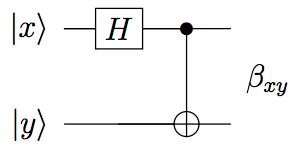
\includegraphics[width=4cm]{Figures/bell}
\end{center}

Es decir, partiendo del estado inicial \( \ket{xy} \), se aplica \textit{H} al primer qubit, y luego se aplica \textit{CNOT} a ambos, donde el primero es el de control (marcado con el punto negro). En otras palabras, este circuito representa la siguiente ecuación:
\[
  \beta_{xy} = CNOT(H \tensor I)\ket{xy}
\]
Las posibles salidas de este circuito, cuando \( x \) e \( y \) varían entre \( 0 \) y \( 1 \) son las siguientes:
\begin{equation*}
  \begin{split}
    \ket{00} \xrightarrow{H(1)} \frac{1}{\sqrt{2}} (\ket{0} + \ket{1})\ket{0} = \frac{1}{\sqrt{2}} (\ket{00} + \ket{10}) \xrightarrow{CNOT(1,2)} \frac{1}{\sqrt{2}} (\ket{00} + \ket{11}) = \beta_{00} \\
    \ket{01} \xrightarrow{H(1)} \frac{1}{\sqrt{2}} (\ket{0} + \ket{1})\ket{1} = \frac{1}{\sqrt{2}} (\ket{01} + \ket{11}) \xrightarrow{CNOT(1,2)} \frac{1}{\sqrt{2}} (\ket{01} + \ket{10}) = \beta_{01} \\
    \ket{10} \xrightarrow{H(1)} \frac{1}{\sqrt{2}} (\ket{0} - \ket{1})\ket{0} = \frac{1}{\sqrt{2}} (\ket{00} - \ket{10}) \xrightarrow{CNOT(1,2)} \frac{1}{\sqrt{2}} (\ket{00} - \ket{11}) = \beta_{10} \\
    \ket{11} \xrightarrow{H(1)} \frac{1}{\sqrt{2}} (\ket{0} - \ket{1})\ket{1} = \frac{1}{\sqrt{2}} (\ket{01} - \ket{11}) \xrightarrow{CNOT(1,2)} \frac{1}{\sqrt{2}} (\ket{01} - \ket{10}) = \beta_{11}
  \end{split}
\end{equation*}

A estos estados se los llama \textit{estados de Bell}. Estos son
estados entrelazados, es decir, estados que no pueden representarse como el producto tensorial de dos estados individuales.

Un par de qubits que se encuentren en un estado de Bell se conoce como \textit{par EPR}. El nombre se debe a que Einstein, Podolsky y Rosen propusieron en 1935 la existencia de un fenómeno por el cual, cuando se tiene un par entrelazado (representado físicamente, por ejemplo, por el spin de un par de electrones o la polarización de un par de fotones) y un estado del par colapsa como resultado de haber realizado una medición, el segundo también colapsará, independientemente de qué tan lejos se encuentren físicamente. Este comportamiento parecía físicamente imposible, por lo cual se lo denominó la \textit{paradoja EPR}. Durante mucho tiempo se pensó que esto se debía a que la formulación de la mecánica cuántica estaba incompleta y que debía ser extendida, pero eventualmente este fenómeno pudo ser verificado experimentalmente.

\subsection{Teleportación cuántica}\label{teleportation}

La teleportación cuántica es un proceso mediante el cual se pueden transmitir qubits de una ubicación a otra mediante la ayuda de la comunicación clásica y de la existencia de un estado de Bell compartido entre el origen y el destino.

Utilizando como ejemplo a los personajes clásicos Alice y Bob, los pasos a seguir son los siguientes:
\begin{enumerate}
  \item Alice y Bob preparan un estado de Bell.
  \item Alice se queda con el primer qubit del par y Bob se lleva el segundo.
  \item Alice aplica \textit{CNOT} entre el qubit a transmitir y su parte del estado de Bell, y luego Hadamard al primero.
  \item Alice realiza una medición sobre los dos qubits en su poder y envía el resultado de la medición (2 bits clásicos) a Bob.
  \item Bob aplica una transformación sobre su qubit, de acuerdo a los bits recibidos: \( Z^{b_1} X^{b_2} \).
\end{enumerate}

El circuito completo queda de la siguiente forma:

\begin{center}
  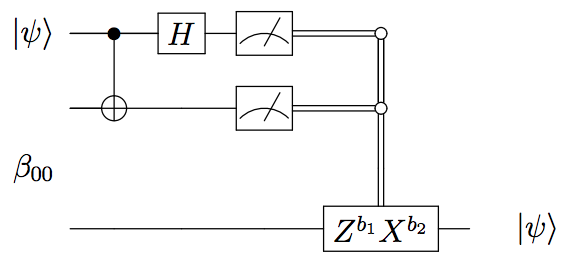
\includegraphics[width=6cm]{Figures/teleportation}
\end{center}

donde \( \ket{\psi} \) es el qubit a transmitir (o ``teleportar'').

Ejemplo: se quiere transmitir el qubit \( \ket{\psi} = \alpha \ket{0} + \beta \ket{1} \), entonces:
\begin{equation*}
  \begin{split}
    \ket{\psi} \tensor \beta_{00}
    & = (\alpha \ket{0} + \beta \ket{1}) \left(\frac{1}{\sqrt{2}} (\ket{0} + \ket{1}) \right) \\
    & = \frac{1}{\sqrt{2}} (\alpha \ket{0} (\ket{00} + \ket{11}) + \beta \ket{1} (\ket{00} + \ket{11})) \\
    & \xrightarrow{CNOT(1,2)} \frac{1}{\sqrt{2}} (\alpha \ket{0} (\ket{00} + \ket{11}) + \beta \ket{1} (\ket{10} + \ket{01})) \\
    & \xrightarrow{H(1)} \frac{1}{\sqrt{2}} \left( \alpha \frac{1}{\sqrt{2}} (\ket{0} + \ket{1})(\ket{00} + \ket{11}) + \beta \frac{1}{\sqrt{2}} (\ket{0} - \ket{1})(\ket{10} + \ket{01}) \right) \\
    & = \frac{1}{2} ( \ket{00} (\alpha \ket{0} + \beta \ket{1}) + \ket{01} (\alpha \ket{1} + \beta \ket{0}) \\
    & + \ket{10} (\alpha \ket{0} - \beta \ket{1}) + \ket{11} (\alpha \ket{1} - \beta \ket{0}) ) \\
    & = \frac{1}{2} \sum\limits_{b_1 = 0}^1 \sum\limits_{b_2 = 0}^1 \ket{b_1 b_2} (X^{b_2} Z^{b_1}) \ket{\psi}
  \end{split}
\end{equation*}

Por lo tanto, aplicando \( Z^{b_1} X^{b_2} \), Bob obtendrá el estado original \( \ket{\psi} \).

\section{\texorpdfstring{\( \lambdacalculus \)}{lambda calculus}}

El \( \lambdacalculus \) es un sistema formal introducido por Alonzo Church en 1930 para estudiar los fundamentos de la lógica y la matemática. Dicho cálculo posee dos simplificaciones que hacen que su semántica sea muy simple. La primera es que las funciones son tratadas como anónimas, es decir, no se les da un nombre. Por ejemplo, la función
\[ \mathsf{incrementar}(x) = x + 1 \]
puede ser reescrita anónimamente como
\[ (x) \mapsto x + 1 \]
Por otra parte, la función
\[ \mathsf{sumar}(x, y) = x + y \]
puede ser reescrita anónimamente como
\[ (x, y) \mapsto x + y \]
La segunda simplificación es que el \( \lambdacalculus \) solo considera funciones que tomen un solo argumento. Para representar funciones que tomen más de un argumento, como \textsf{sumar}, se puede representar como una función que tome un argumento, y como salida devuelva otra función que tome otro argumento. Por ejemplo,
\[ (x, y) \mapsto x + y \]
puede ser reescrita como
\[ x \mapsto (y \mapsto x + y) \]

A pesar de su simpleza, el \( \lambdacalculus \) puede ser utilizado para simular cualquier máquina de Turing. Esto significa que, dado cualquier modelo computacional, existe un equivalente en el \( \lambdacalculus \).
Por ejemplo, para modelar los números naturales y las operaciones sobre ellos, Church diseñó una codificación que lleva su nombre. En los siguientes ejemplos, vamos a asumir la existencia de los números naturales junto con el operador de suma (\( + \)), y al final de la sección mencionaremos cómo se modelan utilizando la codificación de Church.

La gramática de términos en forma BNF del \( \lambdacalculus \) es la siguiente\footnote{Para una introducción a gramáticas formales en \textit{Backus normal form}, ver, por ejemplo: \url{http://www.garshol.priv.no/download/text/bnf.html}}:
\[
  \tag{Términos}
  t \triangleq x \mid (\lambda x . t) \mid (\app{t}{t})
\]
Es decir, se tienen variables, que normalmente se notan utilizando \( x \), \( y \) o \( z \), funciones, que se notan \( \lcabstr{x}{t} \) y aplicaciones de un término \( t \) a otro término \( r \), notado simplemente \( \lcapp{t}{r} \).
Por ejemplo, \textsf{incrementar} se puede escribir en el \( \lambdacalculus \) como
\[ (\lambda x . x + 1) \]
Por otra parte, \textsf{sumar} puede ser escrita como
\[ (\lambda y (\lambda x . x + y)) \]

La gramática nos da la forma de construir términos válidos. Por otro lado, una regla de reescritura o reducción nos dice cómo se interpreta operacionalmente.
La regla de reducción del \( \lambdacalculus \) es la siguiente:
% \[
%   \tag{\(\alpha\text{-conversión}\)}
%   (\abstr{x}{t}[x]) \reducesto (\abstr{y}{t}[y])
% \]
\[
  \tag{\(\beta\text{-reducción}\)}
  ((\lambda x . t) r) \reducesto t [r/x]
\]
Es decir, el término \( \lcapp{\lcabstr{x}{t}}{r} \) puede ser reescrito en el término \( t \), donde todas las ocurrencias de \( r \) son reemplazadas por \( x \).
Por ejemplo, \( \mathsf{incrementar}(3) \) se puede computar como
\[ \lcapp{\lcabstr{x}{x + 1}}{3} \reducesto 3 + 1 \]
Por otra parte, \( \mathsf{sumar}(5, 6) \) se puede computar como
\[ \lcapp{\lcabstr{y}{\lcapp{\lcabstr{x}{x + y}}{5}}}{6} \reducesto \lcapp{\lcabstr{y}{5 + y}}{6} \reducesto 5 + 6 \]

Cabe destacar que en la primera reducción del ejemplo precedente, no se ha utilizado exactamente la regla. Efectivamente, la regla dice cómo reducir \( \lcapp{\lcabstr{x}{t}}{r} \), y en este ejemplo teníamos \( \lcapp{\lcabstr{y}{\lcapp{\lcabstr{x}{x + y}}{5}}}{6} \) para el cual la regla de reducción nos dice que debería reducir en \( \lcapp{\lcabstr{x}{x + 6}}{5} \). Lo que hicimos fue aplicar una regla de contexto. Las reglas de contexto del \( \lambdacalculus \) son las siguientes:
\[
  \quad\quad\quad
  \infer{\lcapp{t}{s} \reducesto \lcapp{r}{s}}{t \reducesto r}
  \quad\quad\quad\quad
  \infer{\lcapp{s}{t} \reducesto \lcapp{s}{r}}{t \reducesto r}
  \quad\quad\quad\quad
  \infer{\lcabstr{x}{t} \reducesto \lcabstr{x}{r}}{t \reducesto r}
\]
Con esta regla, sí podemos reducir \( \lcapp{\lcabstr{y}{\lcapp{\lcabstr{x}{x + y}}{5}}}{6} \) en \( \lcapp{\lcabstr{y}{5 + y}}{6} \), como hicimos en el último ejemplo.

En cuanto a los números naturales, estos pueden ser codificados de la siguiente forma:
\begin{equation*}
  \begin{split}
    0 & \triangleq \lcabstr{f}{\lcabstr{x}{x}} \\
    1 & \triangleq \lcabstr{f}{\lcabstr{x}{\lcapp{f}{x}}} \\
    2 & \triangleq \lcabstr{f}{\lcabstr{x}{\lcapp{f}{\lcapp{f}{x}}}} \\
    & \vdots
  \end{split}
\end{equation*}
Con respecto al operador de suma, este se modela esencialmente como la función que toma dos números codificados de esta forma, y produce la codificación correspondiente a la suma de ellos.

\section{\texorpdfstring{\( \lambdacalculus \)}{lambda calculus} simplemente tipado}

Consideremos el término \( \lcabstr{x}{\lcapp{x}{x}} \) del \( \lambdacalculus \) original, el cual aplicado a un término \( t \), posee el siguiente comportamiento:
\[
  \lcapp{\lcabstr{x}{\lcapp{x}{x}}}{t} \reducesto \lcapp{t}{t}
\]
Ahora consideremos qué ocurre si aplicamos \( (\lambda x . x x) \) a sí mismo:
\[
  \lcapp{\lcabstr{x}{\lcapp{x}{x}}}{\lcabstr{x}{\lcapp{x}{x}}} \reducesto \lcapp{\lcabstr{x}{\lcapp{x}{x}}}{\lcabstr{x}{\lcapp{x}{x}}}
\]
Vemos que al reducir el término \( \lcapp{\lcabstr{x}{\lcapp{x}{x}}}{\lcabstr{x}{\lcapp{x}{x}}} \) volvemos a obtener el mismo, sobre el cuál podemos volver a aplicar la misma regla de reducción. Es evidente que este término puede reescribir infinitamente.

Con el objetivo de excluir ciertos términos del \( \lambdacalculus \) original, en particular los términos que reescriben infinitamente, Alonzo Church introdujo en 1940 una extensión conocida como \textit{lambda cálculo simplemente tipado}. La idea consistía en introducir un sistema que permita asignar tipos a ciertos términos, excluyendo del lenguaje aquellos para los cuales un tipo no pueda ser asignado.

La sintaxis de términos del \( \lambdacalculus \) simplemente tipado es la siguiente:
\[
  \tag{Términos}
  t \triangleq x \mid \stlcabstr{x}{A}{t} \mid \stlcapp{t}{t}
\]
Por ejemplo, la función \textsf{incrementar} de la sección anterior se podría escribir como
\[ \stlcabstr{x}{\mathbb{N}}{x + 1} \]
o bien como
\[ \stlcabstr{x}{\mathbb{R}}{x + 1} \]
dependiendo del conjunto de números sobre la que la queramos definir.

Por otra parte, la sintaxis de tipos es la siguiente:
\[
  A \triangleq \tau \mid A \Rightarrow A \text{ donde } \tau \text{ es un tipo básico y } A \Rightarrow B \text{ el tipo función.}
\]

En cuanto a la semántica operacional, tenemos la siguiente regla de reducción (la cual coincide con la del \( \lambdacalculus \) original ignorando la notación de tipo):
\[
  \stlcapp{\stlcabstr{x}{A}{t}}{r} \reducesto t[r/x]
\]

Por ejemplo, \( \mathsf{incrementar}(3) \) se podría computar como
\[ \stlcapp{\stlcabstr{x}{\mathbb{N}}{x + 1}}{3} \reducesto 3 + 1 \]

Llamamos \textit{contexto} a un conjunto de variables tipadas y lo notamos con \( \Gamma \):
\[
  \Gamma \triangleq \vrbl{x_1}{A_1}, \ldots, \vrbl{x_n}{A_n}
\]

El \( \lambdacalculus \) simplemente tipado posee las siguientes reglas de tipado:

\begin{equation*}
  \infer{\Gamma \vdash x : A}{\vrbl{x}{A} \in \Gamma}
  \quad\quad\quad
  \infer{\Gamma \vdash \stlcabstr{x}{A}{t} : A \Rightarrow B}{\Gamma, \vrbl{x}{A} \vdash t : B}
  \quad\quad\quad
  \infer{\Gamma \vdash \stlcapp{t}{r} : B}{\Gamma \vdash t : A \Rightarrow B & \Gamma \vdash r : A}
\end{equation*}

Por ejemplo, suponiendo que ya sabemos que \( \Gamma \vdash 3 : \mathbb{N} \) y \( \Gamma, x : \mathbb{N} \vdash x + 1 : \mathbb{N} \), para derivar el tipo de la expresión \( \stlcapp{\stlcabstr{x}{\mathbb{N}}{x + 1}}{3} \) procedemos de la siguiente forma:
\[ \infer{\Gamma \vdash \stlcapp{\stlcabstr{x}{\mathbb{N}}{x + 1}}{3} : \mathbb{N}}{\infer{\Gamma \vdash \stlcabstr{x}{\mathbb{N}}{x + 1} : \mathbb{N} \Rightarrow \mathbb{N}}{\Gamma, \vrbl{x}{\mathbb{N}} \vdash x + 1 : \mathbb{N}} & \Gamma \vdash 3 : \mathbb{N}} \]

Por otra parte, no es posible derivar un tipo para la expresión \( \stlcapp{\stlcabstr{x}{\mathbb{N}}{x + 1}}{\pi} \) donde \( \pi : \mathbb{R} \). Esto significa que dicha expresión no es un término válido. Similarmente, es imposible asignarle un tipo a la expresión \( (\lambda x . x x)(\lambda x . x x) \), por lo cual esta expresión no corresponde a un término del \( \lambdacalculus \) simplemente tipado. Lo mismo ocurre con cualquier expresión que en el \( \lambdacalculus \) original resultaba en un término que reescribía infinitamente. Esta propiedad es la que se conoce como \textit{normalización fuerte}, y en el siguiente capítulo vamos a probar su existencia.

\chapter{Normalización fuerte del \texorpdfstring{\( \lambdacalculus \)}{lambda calculus} simplemente tipado}\label{Chapter3}

Vamos a probar que el \( \lambdacalculus \) simplemente tipado posee la propiedad de normalización fuerte, con el objetivo de introducir las técnicas que luego utilizaremos para probar dicha propiedad sobre \( \lambdas \). Esta demostración se basa en la demostración de Tait~\cite{tait}.

Si bien este capítulo se enfoca en el \( \lambdacalculus \) simplemente tipado, en las siguientes definiciones vamos a dar algunos ejemplos del \( \lambdacalculus \) no tipado, con el objetivo de resaltar algunas de las diferencias entre estos dos cálculos en el contexto de la normalización fuerte.

\begin{definition}
  Llamamos \textit{secuencia de reducción} que comienza en \( t \) a una secuencia de términos \( s_1, s_2, \dots \), con \( s_1 = t \) tal que para todo \( s_i, s_{i + 1} \) en la secuencia, \( s_i \reducesto s_{i + 1} \).
\end{definition}
Por ejemplo, \( \lcapp{\lcabstr{y}{\lcapp{\lcabstr{x}{x + y}}{5}}}{6} \), \( \lcapp{\lcabstr{y}{5 + y}}{6} \), \( 5 + 6 \), \( 11 \) es una secuencia de reducción que comienza en \( \lcapp{\lcabstr{y}{\lcapp{\lcabstr{x}{x + y}}{5}}}{6} \),
dado que
\[ \lcapp{\lcabstr{y}{\lcapp{\lcabstr{x}{x + y}}{5}}}{6} \reducesto \lcapp{\lcabstr{y}{5 + y}}{6} \reducesto 5 + 6 \reducesto 11 \]

\begin{definition}
  Decimos que un término \( t \) es \textit{fuertemente normalizante} cuando no existe una secuencia de reducción infinita que comience en \( t \).
\end{definition}

Por ejemplo, en el \( \lambdacalculus \) no tipado, \( \lcapp{ \lcabstr{x}{\lcapp{x}{x}} }{ \lcabstr{x}{\lcapp{x}{x}} } \) no es un término fuertemente normalizante, ya que como vimos, existe una secuencia de reducción infinita que comienza en dicho término. Por otra parte, el término \( \lcapp{\lcabstr{y}{\lcapp{\lcabstr{x}{x + y}}{5}}}{6} \) es fuertemente normalizante ya que cualquier estrategia de reducción termina en \( 11 \) y de ahí no se puede seguir reduciendo.

\begin{definition}
  Dado un término fuertemente normalizante \( t \), notamos \( \lpl{t} \) a la longitud de la secuencia de reducción más larga que comienza en \( t \).
\end{definition}

Por ejemplo, \( \lpl{\lcapp{\lcabstr{y}{\lcapp{\lcabstr{x}{x + y}}{5}}}{6}} = 4 \) y \( \lpl{11} = 1 \).
Por otra parte,
\[  \lpl{\lcapp{\lcabstr{x}{\lcapp{x}{x}}}{\lcabstr{x}{\lcapp{x}{x}}}}
\]
no está definido, dado que \( \lcapp{ \lcabstr{x}{\lcapp{x}{x}} }{ \lcabstr{x}{\lcapp{x}{x}} } \) no es fuertemente normalizante.

\begin{definition}
  Definimos como \( \snset \) al \textit{conjunto de términos fuertemente normalizantes}. Formalmente:
  \[ \snset = \{ t \mid \exists \lpl{t} \} \]
\end{definition}

Por ejemplo, en el \( \lambdacalculus \) no tipado, \( \lcabstr{x}{x} \in \snset \) y \( \lcapp{\lcabstr{y}{5 + y}}{6} \in \snset \) mientras que \( \lcapp{ \lcabstr{x}{\lcapp{x}{x}} }{ \lcabstr{x}{\lcapp{x}{x}} } \notin \snset \).

En el caso del \( \lambdacalculus \) simplemente tipado, vamos a mostrar que todos los términos están en \( \snset \).

\begin{definition}
  Definimos como \( \red{t} \) al conjunto de reductos de \( t \) en un paso. Formalmente:
  \[ \red{t} = \{r \mid t \reducesto r\} \]
\end{definition}

Por ejemplo,
\( \red{\lcapp{\lcabstr{y}{\lcapp{\lcabstr{x}{x + y}}{5}}}{6}} = \{\lcapp{\lcabstr{y}{5 + y}}{6}, \lcapp{\lcabstr{x}{x + 6}}{5}\} \),
ya que existen dos reglas de reducción que podemos aplicar sobre \( \lcapp{\lcabstr{y}{\lcapp{\lcabstr{x}{x + y}}{5}}}{6} \) (la \( \beta \)-reducción normal o la regla contextual).
Por otra parte, \( 5 + 6 \notin \red{\lcapp{\lcabstr{y}{\lcapp{\lcabstr{x}{x + y}}{5}}}{6}} \), ya que se necesitan de dos reducciones para llegar a \( 5 + 6 \).

A partir de aquí, vamos a hablar estrictamente del \( \lambdacalculus \) simplemente tipado.

Ahora vamos a introducir el concepto fundamental de la técnica de Tait para probar normalización fuerte: \textit{reducibilidad}. La idea es introducir una serie de conjuntos de términos muy particulares asociados a cada tipo, definidos de forma tal que se pueda probar que si un término pertenece a dicho conjunto, entonces es fuertemente normalizante. Luego, basta con probar que todo término pertenece al conjunto asociado a su tipo para concluir que todos los términos son fuertemente normalizantes.

\begin{definition}
  Dado un tipo \( A \), definimos \( \interp{A} \) (leído como \textit{interpretación de A}) inductivamente de la siguiente forma:
  \begin{equation*}
    \begin{split}
      \interp{\tau} & = \snset \\
      \interp{\Psi \Rightarrow A} & = \{ t \mid \forall r \in \interp{\Psi}, \stlcapp{t}{r} \in \interp{A} \}
    \end{split}
  \end{equation*}

  Si \( t \in \interp{A} \), decimos que \( t \) es \textit{reducible}.
\end{definition}

A continuación, vamos a enunciar y probar una serie de propiedades fundamentales del concepto de reducibilidad.

Notar que la propiedad CR1 del Lema~\ref{lem:cr-stlc} probará el cierre del conjunto por reducción, y sería interesante poder probar el cierre por antirreducción, es decir, si \( \red{t} \subseteq \interp{A} \) entonces \( t \in \interp{A} \). Sin embargo, probar esto para el caso general es muy difícil. Es por este motivo que Girard~\cite{girard-thesis} introdujo el concepto de \textit{neutralidad}. La idea es que no necesitamos probar la propiedad para el caso general, sino solo para los casos que nos interesan. En efecto, solo necesitamos esta propiedad para las aplicaciones, y para este subconjunto de términos, la prueba es más sencilla.

\begin{definition}
  Llamamos \( \neutralset \) al conjunto de términos \textit{neutrales} compuesto únicamente por las aplicaciones: si \( t \) y \( r \) son términos, entonces \( \stlcapp{t}{r} \in \neutralset \).
\end{definition}

\begin{lemma}\label{lem:cr-stlc}
  Para todo tipo \( A \), se cumplen las siguientes propiedades:
  \begin{description}
    \item[(CR1)] \( \interp{A} \subseteq \snset \)
    \item[(CR2)] Si \( t \in \interp{A} \), entonces \( \red{t} \subseteq \interp{A} \).
    \item[(CR3)] Si \( t \in \neutralset \) y \( \red{t} \subseteq \interp{A} \) entonces \( t \in \interp{A} \).
    \item[(HAB)] Para todo \( x \), \( x \in \interp{A} \).
  \end{description}
\end{lemma}

\begin{proof}
  Procedemos por inducción estructural sobre \( A \):
  \subsection*{\( A = \tau \)}
    \begin{itemize}
      \item CR1
        \\ Por definición, \( \interp{\tau} = \snset \), por lo que efectivamente \( \interp{\tau} \subseteq \snset \).
      \item CR2
        \\ Dado \( t \in \interp{\tau} \), queremos mostrar que \( \red{t} \in \interp{\tau} \). Por definición, \( \interp{\tau} = \snset \), por lo que \( t \in \snset \), y por lo tanto, \( \red{t} \subseteq \snset = \interp{\tau} \), que es lo que queríamos mostrar.
      \item CR3
        \\ Dado \( t \in \neutralset \) donde \( \red{t} \subseteq \interp{\tau} \), queremos mostrar que \( t \in \interp{\tau} \). Por definición de \( \interp{\tau} \), esto equivale a mostrar que \( t \in \snset \).
        \\ Como \( \red{t} \subseteq \interp{\tau} = \snset \), tenemos que \( t \in \snset \), que es lo que queríamos mostrar.
      \item HAB
        \\ Dado \( x \), queremos mostrar que \( x \in \interp{\tau} \). Como \( x \in \snset \), tenemos por definición de \( \interp{\tau} \) que \( x \in \interp{\tau} \), que es lo que queríamos mostrar.
    \end{itemize}
  \subsection*{\( A = \Psi \Rightarrow B \)}
    \begin{itemize}
      \item CR1
        \\ Dado \( t \in \interp{\Psi \Rightarrow B} \), queremos mostrar que \( t \in \snset \).  Sea \( r \in \interp{\Psi} \) (notar que por hipótesis de inducción (HAB), tal \( r \) existe). Por definición, tenemos que \( \stlcapp{t}{r} \in \interp{B} \).
        Y por hipótesis de inducción, tenemos que \( \stlcapp{t}{r} \in \snset \), es decir, \( \lpl{\stlcapp{t}{r}} \) es finito.
        Y como \( \lpl{t} \leq \lpl{\stlcapp{t}{r}} \), tenemos que \( \lpl{t} \) es finito, y por lo tanto, \( t \in \snset \).
      \item CR2
        \\ Dado \( t \in \interp{\Psi \Rightarrow B} \), queremos mostrar que \( \red{t} \in \interp{\Psi \Rightarrow B} \). Si \( \red{t} = \emptyset \), ya estamos. Si no, sea \( t' \in \red{t} \) y \( r \in \interp{\Psi} \).
        Luego \( \stlcapp{t}{r} \in \interp{B} \). Y como \( \stlcapp{t'}{r} \in \red{\stlcapp{t}{r}} \), tenemos por hipótesis de inducción que \( \stlcapp{t'}{r} \in \interp{B} \).
        Luego \( t' \in \interp{\Psi \Rightarrow B} \), que es lo que queríamos mostrar.
      \item CR3
        \\ Dado \( t \in \neutralset \) donde \( \red{t} \subseteq \interp{\Psi \Rightarrow B} \), queremos mostrar que \( t \in \interp{\Psi \Rightarrow B} \). Sea \( r \in \interp{\Psi} \). Queremos mostrar que \( \stlcapp{t}{r} \in \interp{B} \). Por hipótesis de inducción, basta con mostrar que \( \red{\stlcapp{t}{r}} \subseteq \interp{B} \).
        Como \( r \in \interp{\Psi} \), tenemos por hipótesis de inducción (CR1) que \( r \in \snset \), es decir, \( \lpl{r} \) existe. Por lo tanto, podemos proceder por inducción (2) sobre \( \lpl{r} \).
        Analizamos los posibles reductos de \( \stlcapp{t}{r} \):
        \begin{itemize}
          \item \( \stlcapp{t}{r} \reducesto \stlcapp{t'}{r} \) donde \( t \reducesto t' \)
            \\ Como \( t' \in \red{t} \), tenemos que \( t' \in \interp{\Psi \Rightarrow B} \). Y como \( r \in \interp{\Psi} \), tenemos por definición que \( \stlcapp{t'}{r} \in \interp{B} \), que es lo que queríamos mostrar.
          \item \( \stlcapp{t}{r} \reducesto \stlcapp{t}{r'} \) donde \( r \reducesto r' \)
            \\ Como \( r \in \interp{\Psi} \), tenemos por hipótesis de inducción (CR2) que \( r' \in \interp{\Psi} \). Y como \( \lpl{r'} < \lpl{r} \), tenemos por hipótesis de inducción 2 que \( \stlcapp{t}{r'} \in \interp{B} \), que es lo que queríamos mostrar.
        \end{itemize}
        Notar que no puede haber una \( \beta \)-reducción a la cabeza ya que \( t \in \neutralset \), y por definición, las abstracciones no son parte de \( \neutralset \). Este es precisamente el caso difícil que el concepto de neutralidad evita y el motivo por el cual la prueba se simplifica.
      \item HAB
        \\ Dado \( x \), queremos mostrar que \( x \in \interp{\Psi \Rightarrow B} \). Por definición de \( \interp{\Psi \Rightarrow B} \), basta con mostrar que, para todo \( t \in \interp{\Psi} \), tenemos que \( \stlcapp{x}{t} \in \interp{B} \).
        \\ Sea \( t \in \interp{\Psi} \). Por hipótesis de inducción (CR1), tenemos que \( t \in \snset \). Por lo tanto, podemos proceder por inducción (2) sobre \( \lpl{t} \):
        \begin{itemize}
          \item \( \lpl{t} = 1 \)
            \\ En este caso, \( \red{t} = \emptyset \) y por hipótesis de inducción (CR3) tenemos que \( \stlcapp{x}{t} \in \interp{B} \), que es lo que queríamos mostrar.
          \item \( \lpl{t} > 1 \)
            \\ Sea \( \stlcapp{x}{t'} \) tal que \( t \reducesto t' \). Por hipótesis de inducción (2), \( \stlcapp{x}{t'} \in \interp{B} \), es decir, \( \red{\stlcapp{x}{t}} \subseteq \interp{B} \).
            Y como \( \stlcapp{x}{t} \in \neutralset \), tenemos por hipótesis de inducción (CR3) que \( \stlcapp{x}{t} \in \interp{B} \), que es lo que queríamos mostrar.
            \qedhere
        \end{itemize}
    \end{itemize}
\end{proof}

% Ya habiendo probado el teorema de adecuación, vamos a probar que las variables pertenecen a la interpretación de cualquier tipo, lo cual nos permitirá afirmar que la substitución trivial \textsf{Id}, que sustituye cada variable por sí misma, cumple \( \mathsf{Id} \models \Gamma \) para todo \( \Gamma \).

Si podemos probar que todos los términos pertenecen a la interpretación de su tipo (es decir, son reducibles), entonces por Lema~\ref{lem:cr-stlc} (CR1) vamos a tener que todos los términos son fuertemente normalizantes. Esto es lo que vamos a hacer a continuación.

\begin{definition}
  Notamos \( \theta = [r_1/x_1, \ldots, r_n/x_n] \) a las sustituciones de variables por términos, donde cada variable se sustituye por el correspondiente término de manera simultánea.\\
  Dado \( \theta = [r_1/x_1, \ldots, r_k/x_k] \) y \( \theta' = [r_{k + 1}/x_{k + 1}, \ldots, r_n/x_n] \), notamos \( \theta \cup \theta' \) a la sustitución \( [r_1/x_1, \ldots, r_n/x_n] \).\\
  Dado \( \theta \), escribimos \( \theta \models \Gamma \) si para todo \( x : A \in \Gamma \) tenemos que \( \theta(x) \in \interp{A} \). Por otra parte, si \( y \) no está en \( \Gamma \), \( \theta(y) = y \).
\end{definition}

\begin{lemma}[Adecuación]\label{lem:adequacy-stlc}
  Si \( \Gamma \vdash t:A \) y \( \theta \models \Gamma \) entonces \( \theta(t) \in \interp{A} \).
\end{lemma}

\begin{proof}
  Procedemos por inducción estructural sobre la derivación de \( \Gamma \vdash t : A \):
  \begin{itemize}
    \item \( \infer{\Gamma \vdash x : A}{x : A \in \Gamma} \)
      \\ Trivial.
    \item \( \infer{\Gamma \vdash \abstr{x : A}{t} : A \Rightarrow B}{\Gamma, x : A \vdash t : B} \)
      \\ Nuestra hipótesis de inducción dice que si \( \theta \models \Gamma, x : A \), entonces \( \theta(t) \in \interp{B} \).
      Queremos mostrar que si \( \theta' \models \Gamma \), entonces \( \theta'(\abstr{x : A}{t}) = (\abstr{x : A}{\theta'(t)}) \in \interp{A \Rightarrow B} \), o lo que es lo mismo, para todo \( r \in \interp{A}, \app{(\abstr{x : A}{\theta'(t)})}{r} \in \interp{B} \).
      \\ Como \( \app{(\abstr{x : A}{\theta'(t)})}{r} \in \neutralset \), el Lema~\ref{lem:cr-stlc} (CR3) nos dice que si \( \red{\app{(\abstr{x : A}{\theta'(t)})}{r}} \subseteq \interp{B} \), entonces \( \app{(\abstr{x : A}{\theta'(t)})}{r} \in \interp{B} \). Vamos a mostrar que efectivamente \( \red{\app{(\abstr{x : A}{\theta'(t)})}{r}} \subseteq \interp{B} \).
      \\ Como \( \theta'(t) = (\theta' \circ [x/x])(t) \) y \( (\theta' \circ [x/x]) \models \Gamma, x : A \), tenemos por hipótesis de inducción que \( \theta'(t) \in \interp{B} \). Y como \( r \in \interp{A} \), tenemos por Lema~\ref{lem:cr-stlc} (CR2) que ambos términos son fuertemente normalizantes. Por lo tanto, podemos proceder por inducción (2) sobre \( |\theta'(t)| + |r| \). Analizamos cada uno de los reductos de \( \app{(\abstr{x : A}{\theta'(t)})}{r} \):
      \begin{itemize}
        \item \( \app{(\abstr{x : A}{\theta'(t)})}{r} \reducesto \theta'(t)[r/x] \)
        \\ Queremos mostrar que \( \theta'(t)[r/x] \in \interp{B} \). Por definición, \( \theta'(t)[r/x] = (\theta' \circ [r/x])(t) \), y como \( r \in \interp{A} \), tenemos \( (\theta' \circ [r/x]) \models \Gamma, x:A \). Por lo tanto, por hipótesis de inducción, tenemos que \( \theta'(t)[r/x] \in \interp{B} \), que es lo que queríamos mostrar.
        \item \( \app{(\abstr{x : A}{\theta'(t)})}{r} \reducesto \theta(\abstr{x : A}{s}) r \) donde \( \theta'(t) \reducesto s \)
        \\ Queremos mostrar que \( \app{(\abstr{x : A}{s})}{r} \in \interp{B} \). Por hipótesis de inducción 2, \( \app{(\abstr{x : A}{s})}{r} \in \interp{B} \), que es lo que queríamos mostrar.
        \item \( \app{(\abstr{x : A}{\theta'(t)})}{r} \reducesto \app{(\abstr{x : A}{\theta'(t)})}{r'} \)
        \\ Queremos mostrar que \( \app{(\abstr{x : A}{\theta'(t)})}{r'} \in \interp{B} \). Por hipótesis de inducción 2, \( \app{(\abstr{x : A}{\theta'(t)})}{r'} \in \interp{B} \), que es lo que queríamos mostrar.
      \end{itemize}
    \item \( \infer{\Gamma \vdash \app{t}{r} : B}{\Gamma \vdash t : A \Rightarrow B & \Gamma \vdash r : A} \)
      \\ Nuestra hipótesis de inducción dice que si \( \theta \models \Gamma \), entonces \( \theta(t) \in \interp{A \Rightarrow B} \) y \( \theta(u) \in \interp{A} \).
      Queremos mostrar que si \( \theta \models \Gamma \), entonces \( \theta(\app{t}{u}) = \app{\theta(t)}{\theta(u)} \in \interp{B} \).
      \\ Por hipótesis de inducción y definición de \( \interp{A \Rightarrow B} \), tenemos que \( \app{\theta(t)}{\theta(u)} \in \interp{B} \), que es lo que queríamos mostrar.
      \qedhere
  \end{itemize}
\end{proof}

Ahora estamos en condiciones de probar el teorema de normalización fuerte.

\begin{theorem}[Normalización fuerte]
  Si \( \Gamma \vdash t : A \), entonces \( t \in \snset \).
\end{theorem}

\begin{proof}
  Por Lema~\ref{lem:adequacy-stlc}, si \( \theta \models \Gamma \) entonces \( \theta(t) \in \interp{A} \). Por otra parte, por Lema~\ref{lem:cr-stlc} (CR1), tenemos que \( \interp{A} \subseteq \snset \).
  Finalmente, por Lema~\ref{lem:cr-stlc} (HAB), tenemos que \( \mathsf{Id} \models \Gamma \).
  Por lo tanto, \( \mathsf{Id}(t) = t \in \snset \), que es lo que queríamos mostrar.
\end{proof}

\chapter{Introducción a \texorpdfstring{\( \lambdas \)}{Lambda S}}\label{Chapter4}

\( \lambdas \) es una extensión del \( \lambdacalculus \) para modelar la computación cuántica. Este lenguaje utiliza un sistema de tipos inspirado por la lógica lineal~\cite{abramsky} que le permite diferenciar
entre las superposiciones y los estados de la base canónica con el objetivo de cumplir con el teorema del no clonado (Teorema~\ref{thm:no-cloning}). Por otra parte, \( \lambdas \) introduce un sistema de reescritura inspirado por el álgebra lineal~\cite{arrighi3, arrighi4}, el cual le permite tratar a las expresiones que esperan información duplicable como funciones lineales, con el fin de soportar fácilmente el operador de medición.

\section{Gramática de tipos}

La gramática de tipos es la siguiente:
\begin{align*}
	\mathfrak{B} & \triangleq \qubittype \mid \qubittype \times \mathfrak{B} \tag*{Tipos qubit base (\( \mathbf{B} \))} \\
	\Psi         & \triangleq \mathfrak{B} \mid S(\Psi) \mid \Psi \times \Psi \tag*{Tipos qubit (\( \mathbf{Q} \))}       \\
	A            & \triangleq \Psi \mid \Psi \Rightarrow A \mid S(A) \tag*{Tipos (\( \mathbf{T} \))}
\end{align*}
La gramática está dividida en tres niveles: \( \mathfrak{B} \) es para los qubits base, \( \Psi \) se utiliza para qubits generales, y \( A \) para tipos generales.
El tipo \( \qubittype \) se utiliza para los estados base de 1 qubit, como \( \ket{0} \). Si \( \Psi \) es una base, \( S(\Psi) \) se utiliza para el espacio generado por ese conjunto, lo que permite representar superposiciones. Como el tensor de los espacios es lo mismo que el espacio generado por el producto cartesiano de las bases, basta con introducir el constructor \( \times \) para representar el producto tensorial. Notamos \( \underbrace{\qubittype \times \qubittype \times \cdots \times \qubittype}_{n \text{ veces}} \) como \( \qubittype^n \), donde dicho producto asocia a derecha. Por ejemplo, \( \ket{0} \times \ket{1} \) tiene tipo \( \qubittype^2 \), mientras que \( \frac{1}{\sqrt{2}} \ket{0} \times \ket{0} + \frac{1}{\sqrt{2}} \ket{1} \times \ket{1} \) tiene tipo \( S(\qubittype^2) \).

\section{Gramática de pre-términos}

Empezamos por definir la gramática que nos permitirá construir expresiones del lenguaje. A estas expresiones las denominamos \textit{pre-términos}.

La gramática de pre-términos es la siguiente:
\begin{align*}
	b & \triangleq x \mid \abstr{\vrbl{x}{\Psi}}{t} \mid \ket{0} \mid \ket{1} \mid b \times b \tag*{Términos base \( (\mathcal{B}) \)}                                                                       \\
	v & \triangleq b \mid (v + v) \mid \nullvec{A} \mid \alpha . v \mid v \times v \tag*{Valores \( (\mathcal{V}) \)}                                                                                  \\
	t & \triangleq v \mid \app{t}{t} \mid \proj{j}{t} \mid \ifte{}{t}{t} \mid \alpha . t \mid t \times t \mid \head{t} \mid \tail{t} \mid \cast{S(A)}{S(B \times C)} t \tag*{Términos \( (\Lambda) \)}
\end{align*}

La gramática está dividida en tres niveles: \( b \) es para los pre-términos base (valores no superpuestos), \( v \) son los valores generales y \( t \) los pre-términos generales.
Como vimos antes, el constructor \( \times \) se utiliza para representar productos tensoriales. Por ejemplo, \( \ket{01} \) se representa en \( \lambdas \) como \( \ket{0} \times \ket{1} \). El constructor \( \ifte{}{}{} \) se utiliza como un \textit{if-then-else} que decide sobre vectores base. Utilizamos la notación \( \ifte{t}{r}{s} \) para representar \( \app{(\ifte{}{r}{s})}{t} \).
\( \proj{j} \) se utiliza para las mediciones, donde \( j \) representa la cantidad de qubits a medir, los cuales ocupan las primeras \( j \) posiciones. También tenemos los operadores de listas \textsf{head} y \textsf{tail}, y un operador de casting que desarrollaremos más adelante.

A continuación, presentaremos las reglas que nos permitirán asignarles tipos a los pre-términos.

\section{Relación de subtipado}
Un tipo \( A \) es interpretado como un conjunto de vectores, y \( S(A) \) como el espacio vectorial generado por tal conjunto. Es decir que, interpretados como conjuntos de vectores, tenemos que \( A \subseteq S(A) \) y \( S(S(A)) = S(A) \). Por lo tanto, para capturar este fenómeno, podemos establecer la siguiente relación de subtipado:
\[
	\quad\quad\quad\quad\quad\quad\quad\quad
	\infer{A \preceq A}{}
	\quad\quad\quad\quad
	\infer{A \preceq C}{A \preceq B & B \preceq C}
\]
\[
	\quad\quad\quad\quad
	\infer{A \preceq S(A)}{}
	\quad\quad
	\infer{S(S(A)) \preceq S(A)}{}
	\quad\quad
	\infer{\Psi \Rightarrow A \preceq \Psi \Rightarrow B}{A \preceq B}
\]

\[
	\quad\quad\quad
	\infer{S(A) \preceq S(B)}{A \preceq B}
	\quad\quad
	\infer{A \times C \preceq B \times C}{A \preceq B}
	\quad\quad
	\infer{C \times A \preceq C \times B}{A \preceq B}
\]

\section{Sistema de tipos}
El sistema de tipos está compuesto por juicios de la forma \( \Gamma \vdash t:A \), donde \( \Gamma \) es un conjunto de variables tipadas con tipos qubit. En cuanto a dichos conjuntos, se van a obviar las llaves, por lo que se escribirá \( \vrbl{x_1}{\Psi_1},\ldots,\vrbl{x_n}{\Psi_n} \) en lugar de \( \{\vrbl{x_1}{\Psi_1},\ldots,\vrbl{x_n}{\Psi_n}\} \).
\\Las reglas del sistema de tipos son las siguientes:
\[
	\infer[A_X]{\vrbl{x}{\Psi} \vdash x : \Psi}{}
	\quad
	\infer[A_{X_{\vec{0}}}]{\vdash \nullvec{A}: S(A)}{}
	\quad
	\infer[A_{X_{\ket{0}}}]{\vdash \ket{0}: \qubittype}{}
	\quad
	\infer[A_{X_{\ket{1}}}]{\vdash \ket{1}: \qubittype}{}
\]
\[
	\infer[S^{\alpha}_{I}]{\Gamma \vdash \alpha . t : S(A)}{\Gamma \vdash t: A}
	\quad
	\infer[S^{+}_{I}]{\Gamma, \Delta \vdash (t + u): S(A)}{\Gamma \vdash t : A & \Delta \vdash u : A & \Gamma \cap \Delta = \emptyset}
	\quad
	\infer[S_E]{\Gamma \vdash \proj{j}{t} : \qubittype^j \times S(\qubittype^{n - j})}{\Gamma \vdash t : S(\qubittype^n)}
\]
\[
	\infer[\preceq]{\Gamma \vdash t : B}{\Gamma \vdash t: A & A \preceq B}
	\quad
	\infer[\textit{If}]{\Gamma \vdash \ifte{}{t}{r}: \qubittype \Rightarrow A}{\Gamma \vdash t : A & \Gamma \vdash r : A}
	\quad
	\infer[\Rightarrow_I]{\Gamma \vdash \abstr{\vrbl{x}{\Psi}}{t} : \Psi \Rightarrow A}{\Gamma, \vrbl{x}{\Psi} \vdash t : A}
\]
\[
	\quad\quad\quad\quad\quad
	\infer[\Rightarrow_E]{\Gamma, \Delta \vdash \app{t}{u} : A}{\Gamma \vdash t : \Psi \Rightarrow A & \Delta \vdash u : \Psi & \Gamma \cap \Delta = \emptyset}
\]
\[
	\quad\quad\quad\quad\quad
	\infer[\Rightarrow_{ES}]{\Gamma, \Delta \vdash t u : S(A)}{\Gamma \vdash t : S(\Psi \Rightarrow A) & \Delta \vdash u : S(\Psi) & \Gamma \cap \Delta = \emptyset}
\]
\[
	\quad\quad\quad\quad\quad
	\infer[\textit{W}]{\Gamma, \vrbl{x}{\qubittype^n} \vdash t : A}{\Gamma \vdash t: A & x \notin \Gamma}
	\quad
	\infer[\textit{C}]{\Gamma, \vrbl{x}{\qubittype^n} \vdash t[x/y] : A}{\Gamma, \vrbl{x}{\qubittype^n}, \vrbl{y}{\qubittype^n} \vdash t : A}
\]
\[
	\infer[\times_I]{\Gamma, \Delta \vdash t \times u : A \times B}{\Gamma \vdash t : A & \Delta \vdash u : B & \Gamma \cap \Delta = \emptyset}
	\quad
	\infer[\times_{Er}]{\Gamma \vdash head\ t : \qubittype}{\Gamma \vdash t : \qubittype^n}
	\quad
	\infer[\times_{El}]{\Gamma \vdash tail\ t : \qubittype^{n - 1}}{\Gamma \vdash t : \qubittype^n}
\]
\[
	\quad\quad
	\infer[\Uparrow_r]{\Gamma \vdash \cast{S(S(A) \times B)}{S(A \times B)} t : S(A \times B)}{\Gamma \vdash t : S(S(A) \times B)}
	\quad
	\infer[\Uparrow_l]{\Gamma \vdash \cast{S(A \times S(B))}{S(A \times B)} t : S(A \times B)}{\Gamma \vdash t : S(A \times S(B))}
\]

Antes de pasar a explicar las reglas, introducimos la siguiente definición.

\begin{definition}
	Definimos \textit{término} a aquellos pre-términos a los que se les puede asignar un tipo utilizando las reglas precedentes.
\end{definition}

La regla \( A_X \) permite tipar a las variables solo con tipos qubit.

La regla \( A_{X_{\vec{0}}} \) tipa al vector nulo como un término no base, dado que el vector nulo no puede pertenecer a la base de ningún espacio vectorial.

Las reglas \( A_{X_{\ket{0}}} \) y \( A_{X_{\ket{1}}} \) tipan a los qubits base con el tipo base \( \mathbb{B} \).

La regla \( S_I^\alpha \) dice que un término multiplicado por un escalar no es un término base. Esto se debe a que nuestro operador de medición remueve cualquier escalar, por lo que tener uno implica que el término aún no ha sido medido. La regla \( S_I^+ \) es el análogo para sumas de la regla anterior.

La regla \( S_E \) fuerza que el término a medir esté tipado con un tipo de la forma \( S(\qubittype^n) \), y luego de medir los primeros \( j \) qubits, el nuevo tipo pasa a ser \( \qubittype^j \times S(\qubittype^{n - j}) \), es decir, elimina la superposición de los primeros \( j \) tipos en el producto tensorial.

La regla \( \preceq \) es la que permite aplicar las reglas de subtipado sobre los términos.

La regla \textit{If} tipa los términos de la forma \( \ifte{}{t}{r} \) como funciones que esperan argumentos no lineales. Esto implica que el \textit{if-then-else} distribuye linealmente sobre superposiciones. Por ejemplo:
\begin{equation*}
	\begin{split}
		\ifte{(\alpha . \ket{0} + \beta . \ket{1})}{t}{r}
		& = \app{(\ifte{}{t}{r})}{(\alpha . \ket{0} + \beta . \ket{1})} \\
		& \reducesto^* \alpha . \app{(\ifte{}{t}{r})}{\ket{0}} + \beta . \app{(\ifte{}{t}{r})}{\ket{1}} \\
		& = \alpha . \ifte{\ket{0}}{t}{r} + \beta . \ifte{\ket{1}}{t}{r} \\
		& \reducesto^* \alpha . r + \beta . t
	\end{split}
\end{equation*}

La regla \( \Rightarrow_I \) nos dice cómo tipar abstracciones.

La regla \( \Rightarrow_E \) nos dice cómo tipar aplicaciones con términos no superpuestos, mientras que la regla \( \Rightarrow_{ES} \) hace lo mismo sobre superposiciones.

Las reglas \( W \) y \( C \) corresponden a las reglas de weakening y contraction de variables con tipos base, considerando que los términos base se pueden clonar.

Las reglas \( \times_I \), \( \times_{Er} \) y \( \times_{El} \) son la introducción y eliminación estándares para listas.

Las reglas \( \Uparrow_r \) y \( \Uparrow_l \) son los casteos de tipo, donde los únicos casteos posibles son \( S(S(A) \times B) \) y \( S(A \times S(B)) \) en \( S(A \times B) \).

Vamos a introducir una notación especial para combinaciones lineales de términos, que nos será de utilidad para el sistema de reescritura y durante la prueba de normalización fuerte.

\begin{definition}
	Dado un conjunto de términos \( r_1, \ldots, r_n \) y \( n \geq 1 \), notamos \( \sum\limits_{i = 1}^n [\alpha_i .] r_i \) al término \( [\alpha_1 .] r_1 + \cdots + [\alpha_n .] r_n \), donde \( [\alpha_k .] \) indica que \( \alpha_k \) puede no estar presente. \\
	En particular, para \( n = 0 \) y \( r_i \) de tipo \( A \) para todo \( i \), \( \sum\limits_{i = 1}^n [\alpha_i .] r_i = \nullvec{A} \).
\end{definition}

\section{Sistema de reescritura}
El sistema de reescritura posee las siguientes reglas (notar que algunas son dependientes del tipo del término sobre el cual se apliquen, por lo cual el sistema solo está definido sobre términos correctamente tipados):

\textbf{Beta}
\begin{align*}
	\text{Si } b \text{ tiene tipo } \qubittype^n\text{ y } b \in \mathcal{B} \text{, entonces } \app{(\abstr{\vrbl{x}{\qubittype^n}}{t})}{b} \reducesto_{(1)} t[b/x] \tag{\( \beta_\mathsf{b} \)} \\
	\text{Si } u \text{ tiene tipo } S(\Psi) \text{, entonces }
	\app{(\abstr{\vrbl{x}{S(\Psi)}}{t})}{u} \reducesto_{(1)} t[u/x] \tag{\( \beta_\mathsf{n} \)}
\end{align*}

\textbf{If}
\begin{align*}
	\ifte{\ket{1}}{u}{v} & \reducesto_{(1)} u \tag{\( \mathsf{if_1} \)} \\
	\ifte{\ket{0}}{u}{v} & \reducesto_{(1)} v \tag{\( \mathsf{if_0} \)}
\end{align*}

\textbf{Distribuciones lineales}
\begin{align*}
	\text{Si } t \text{ tiene tipo } \qubittype^n \Rightarrow A \text{, entonces } \app{t}{(u + v)}                & \reducesto_{(1)} (\app{t}{u} + \app{t}{v}) \tag{\( \mathsf{lin_r}^+ \)} \\
	\text{Si } t \text{ tiene tipo } \qubittype^n \Rightarrow A \text{, entonces } \app{t}{(\alpha . u)}           & \reducesto_{(1)} \alpha . \app{t}{u} \tag{\( \mathsf{lin_r}^\alpha \)}  \\
	\text{Si } t \text{ tiene tipo } \qubittype^n \Rightarrow A \text{, entonces } \app{t}{\nullvec{\qubittype^n}} & \reducesto_{(1)} \nullvec{A} \tag{\( \mathsf{lin_r}^0 \)}               \\
	\app{(t + u)}{v}                                                                                               & \reducesto_{(1)} (\app{t}{v} + \app{u}{v}) \tag{\( \mathsf{lin_l}^+ \)} \\
	\app{(\alpha . t)}{u}                                                                                          & \reducesto_{(1)} \alpha . \app{t}{u} \tag{\( \mathsf{lin_l}^\alpha \)}  \\
	\app{\nullvec{\qubittype^n \Rightarrow A}}{t}                                                                  & \reducesto_{(1)} \nullvec{A} \tag{\( \mathsf{lin_l}^0 \)}
\end{align*}

\textbf{Axiomas de espacios vectoriales}
\begin{align*}
	\nullvec{S(A)}                                              & \reducesto_{(1)} \nullvec{A} \tag{\textsf{null}}                           \\
	(\nullvec{A} + t)                                           & \reducesto_{(1)} t \tag{\textsf{neutral}}                                  \\
	1 . t                                                       & \reducesto_{(1)} t \tag{\textsf{unit}}                                     \\
	\text{Si } t \text{ tiene tipo } A \text{, entonces } 0 . t & \reducesto_{(1)} \nullvec{A} \tag{\( \mathsf{zero}_\alpha \)}              \\
	\alpha . \nullvec{A}                                        & \reducesto_{(1)} \nullvec{A} \tag{\textsf{zero}}                           \\
	\alpha . (\beta . t)                                        & \reducesto_{(1)} (\alpha \cross \beta) . t \tag{\textsf{prod}}             \\
	\alpha . (t + u)                                            & \reducesto_{(1)} (\alpha . t + \alpha . u) \tag{\( \alpha\mathsf{dist} \)} \\
	(\alpha . t + \beta . t)                                    & \reducesto_{(1)} (\alpha + \beta) . t \tag{\textsf{fact}}                  \\
	(\alpha . t + t)                                            & \reducesto_{(1)} (\alpha + 1) . t \tag{\( \mathsf{fact}^1 \)}              \\
	(t + t)                                                     & \reducesto_{(1)} 2 . t \tag{\( \mathsf{fact}^2 \)}
\end{align*}

\textbf{Igualdades}
\begin{align*}
	(u + v)               & =_{AC} (v + u) \tag{\textsf{comm}}                             \\
	((u + v) + w)         & =_{AC} (u + (v + w)) \tag{\(\mathsf{assoc}^+\)}                \\
	(u \times v) \times w & =_{AC} u \times (v \times w) \tag{\(\mathsf{assoc}^{\times}\)}
\end{align*}

\textbf{Listas}
\begin{align*}
	\text{Si } h \neq u \times v \text{ y } h \in \mathcal{B} \text{, entonces } \head{h \times t} & \reducesto_{(1)} h \tag{\textsf{head}} \\
	\text{Si } h \neq u \times v \text{ y } h \in \mathcal{B} \text{, entonces } \tail{h \times t} & \reducesto_{(1)} h \tag{\textsf{tail}}
\end{align*}

\textbf{Casteos de tipos}
\begin{align*}
	\cast{S(S(A) \times B)}{S(A \times B)} ((r + s) \times u)      & \reducesto_{(1)} (\cast{S(S(A) \times B)}{S(A \times B)}\!(r \times u) + \cast{S(S(A) \times B)}{S(A \times B)}\!(s \times u)) \tag{\( \mathsf{dist_r}^+ \)} \\
	\cast{S(B \times S(A))}{S(B \times A)} (u \times (r + s))      & \reducesto_{(1)} (\cast{S(B \times S(A))}{S(B \times A)}\!(u \times r) + \cast{S(B \times S(A))}{S(B \times A)}\!(u \times s)) \tag{\( \mathsf{dist_l}^+ \)} \\
	\cast{S(S(A) \times B)}{S(A \times B)} ((\alpha . r) \times u) & \reducesto_{(1)} \alpha . \cast{S(S(A) \times B)}{S(A \times B)} (r \times u) \tag{\( \mathsf{dist_r}^\alpha \)}                                             \\
	\cast{S(B \times S(A))}{S(B \times A)} (u \times (\alpha . r)) & \reducesto_{(1)} \alpha . \cast{S(B \times S(A))}{S(B \times A)} (u \times r) \tag{\( \mathsf{dist_l}^\alpha \)}                                             \\
	\cast{S(S(A) \times B)}{S(A \times B)} (\nullvec{A} \times u)  & \reducesto_{(1)} \nullvec{A \times B} \tag{\( \mathsf{dist_r}^0 \)}                                                                                          \\
	\cast{S(B \times S(A))}{S(B \times A)} (u \times \nullvec{A})  & \reducesto_{(1)} \nullvec{B \times A} \tag{\( \mathsf{dist_l}^0 \)}                                                                                          \\
	\cast{S(A)}{S(B \times C)} (t + u)                             & \reducesto_{(1)} (\cast{S(A)}{S(B \times C)} t + \cast{S(A)}{S(B \times C)} u) \tag{\( \mathsf{dist}_\Uparrow^+ \)}                                          \\
	\cast{S(A)}{S(B \times C)} (\alpha . t)                        & \reducesto_{(1)} \alpha \cast{S(A)}{S(B \times C)} t \tag{\( \mathsf{dist}_\alpha^+ \)}
\end{align*}
\begin{align*}
	\text{Si } u \in \mathcal{B} \text{, entonces } \cast{S(S(A) \times B)}{S(A \times B)} (u \times v) & \reducesto_{(1)} u \times v \tag{\( \mathsf{neut_r}^\Uparrow \)} \\
	\text{Si } u \in \mathcal{B} \text{, entonces } \cast{S(A \times S(B))}{S(A \times B)} (v \times u) & \reducesto_{(1)} v \times u \tag{\( \mathsf{neut_l}^\Uparrow \)}
\end{align*}

\textbf{Proyección}
\begin{multline*}
	\proj{j}{(\sum\limits_{i = 1}^n [\alpha_i .] \prod_{h = 1}^m b_{hi})} \reducesto_{(p)} \prod_{h = 1}^j b_{hk} \times \sum\limits_{i \in P} \left(\frac{\alpha_i}{\sqrt{\sum_{r \in P} |\alpha_r|^2}}\right) . \prod_{h = j + 1}^m b_{hi} \text{ donde } k \leq n; \\
	j\!\leq m; P\!\subseteq \mathbb{N}^{\leq n} \mid \forall i\!\in P, \forall h\!\leq j, b_{hi} = b_{hk}; p\!=\!\sum_{i \in P}\!\left( \frac{|\alpha_i|^2}{\sum_{r = 1}^n |\alpha_r|^2}\!\right);
	\forall i, b_i\!\in \{\ket{0},\!\ket{1}\} \\ \sum_{i = 1}^n [\alpha_i .] \prod_{h = 1}^m b_{hi} \text{ es un término normal; y si un } \alpha_k \text{ no aparece, } \alpha_k = 1
	\tag{\textsf{proj}}
\end{multline*}

\textbf{Reglas contextuales}
\[
	\quad\quad\quad\quad\quad\quad
	\infer{\app{t}{v} \reducesto_{(p)} \app{u}{v}}{t \reducesto_{(p)} u}
	\quad\quad
	\infer{\app{(\abstr{\vrbl{x}{\qubittype^n}}{v})}{t} \reducesto_{(p)} \app{(\abstr{\vrbl{x}{\qubittype^n}}{v})}{u}}{t \reducesto_{(p)} u}
\]
\[
	\infer{t + v \reducesto_{(p)} u + v}{t \reducesto_{(p)} u}
	\quad
	\infer{\alpha . t \reducesto_{(p)} \alpha . u}{t \reducesto_{(p)} u}
	\quad
	\infer{\proj{j}{t} \reducesto_{(p)} \proj{j}{u}}{t \reducesto_{(p)} u}
	\quad
	\infer{t \times v \reducesto_{(p)} u \times v}{t \reducesto_{(p)} u}
	\quad
	\infer{v \times t \reducesto_{(p)} v \times u}{t \reducesto_{(p)} u}
\]
\[
	\infer{\ifte{t}{r}{s} \reducesto_{(p)} \ifte{u}{r}{s}}{t \reducesto_{(p)} u}
	\quad
	\infer{\head{t} \reducesto_{(p)} \head{u}}{t \reducesto_{(p)} u}
	\quad
	\infer{\tail{t} \reducesto_{(p)} \tail{u}}{t \reducesto_{(p)} u}
	\quad
	\infer{\cast{S(A)}{S(B)} t \reducesto_{(p)} \cast{S(A)}{S(B)} u}{t \reducesto_{(p)} u}
\]

La relación \( \reducesto_{(p)} \) es probabilística, es decir, corresponde a un conjunto de ternas \( (t, r, p) \) donde \( t \) reduce a \( r \) y \( p \) es la probabilidad de ocurrencia. A excepción de la regla de proyección \textsf{proj}, todas las demás reglas tienen probabilidad de ocurrencia \( 1 \). De ahora en más, cuando conocer \( p \) no sea estrictamente necesario, vamos a escribir \( \reducesto \) para referirnos a \( \reducesto_{(p)} \). A los efectos de demostrar esta propiedad, los \( p \) no son importantes. En la literatura, existen varias nociones diferentes de normalización para lenguajes probabilísticos. Por un lado, tenemos la noción de \textit{terminación casi asegurada} (\textit{almost-surely terminating} o AST en inglés)~\cite{ast}, la cual en principio no impide la posibilidad de que las secuencias de reducción diverjan, pero la probabilidad de que esto ocurra es 0, lo que implica que en el límite las secuencias terminarán. Por otra parte, existe una versión \textit{débil} de la noción anterior (W-AST), la cual pide que exista al menos una secuencia que normalice en el límite. La propiedad de normalización fuerte que se trata en este trabajo implica la AST, la cual a su vez implica la W-AST, por lo que la que vamos a probar aquí es la más fuerte de todas.

El sistema de reescritura depende del tipo de los términos sobre los que se aplique. Por ejemplo, en el caso de las abstracciones, estas pueden esperar un término base o una superposición, teniendo diferentes reglas de reducción para cada caso.

La regla de reducción \( \beta_b \) solo se aplica cuando el argumento de la abstracción es un término base, y el tipo que espera la abstracción es un tipo base, mientras que la regla de reducción \( \beta_n \) espera una superposición.

El grupo \textit{If} representa los tests sobre los qubits base \( \ket{0} \) y \( \ket{1} \).

Las tres primeras del grupo de distribuciones lineales son las reglas que se usan cuando una abstracción a argumento no lineal es aplicada sobre un argumento lineal, es decir, cuando una abstracción esperando un término base obtiene una superposición. En estos casos, las \( \beta \)-reducciones no se pueden aplicar porque las condiciones de tipos no se cumplen. El resto de las reglas de este grupo tratan con superposiciones de funciones. Por ejemplo, la regla \( \mathsf{lin_l}^+ \) es la suma de funciones: una superposición es una suma, por lo tanto, un argumento que se le provee a una suma de funciones debe ser proveído a cada función en la suma.

Las reglas de axiomas de espacios vectoriales representan los axiomas que su nombre indica. Por otra parte, las reglas de igualdades no son reglas de reducción propiamente dichas, sino que expresan el hecho de que el símbolo \( + \) es asociativo y conmutativo.

Las regla \textsf{head} reduce un producto de términos en el primero de ellos, mientras que la regla \textsf{tail} reduce un producto de términos en todos menos el primero, y solo se pueden aplicar si el primer término del producto es un término base.

Las primeras 6 reglas de casteos de tipos tratan con la distributividad de la suma, el producto escalar y el vector nulo. Por ejemplo, la regla \( \mathsf{dist}_r^+ \) actúa sobre el término \( ((r + s) \times u) \), distribuyendo el producto sobre la suma, y produciendo el término \( (r \times u) + (s \times u) \). Sin embargo, el término \( ((r + s) \times u) \) puede tener tipo \( S(A) \times B \), \( S(A) \times S(B) \) o \( S(A \times B) \), mientras que el término \( (r \times u) + (s \times u) \) solo puede tener tipo \( S(A \times B) \), por lo cual no podemos reducir el término directamente. Es por este motivo que \( \lambdas \) introduce el operador de casteo, mediante el cual se transforma el tipo del término de manera explícita para poder reducir.

Las siguientes dos reglas distribuyen el cast con respecto a la suma y a los escalares. Las últimas dos reglas del grupo permiten remover el cast cuando ya no es necesario.

La regla de proyección (\textsf{proj}) es la que permite realizar mediciones. Toma un argumento \( j \) el cual representa la cantidad de qubits a medir y solo actúa sobre términos en forma normal. Esta regla es la única con probabilidad distinto de \( 1 \), y viene dada por el cuadrado del módulo de los pesos. Por ejemplo, dado el término
\[ (2.(\ket{0} \times \ket{1} \times \ket{1}) + (\ket{0} \times \ket{1} \times \ket{0})) + 3.(\ket{1} \times \ket{1} \times \ket{1}) \]
medir los primeros 2 qubits producirá
\[ \ket{0} \times \ket{1} \times (\frac{2}{\sqrt{5}} .\!\ket{1} + \frac{1}{\sqrt{5}} .\!\ket{0}) \text{ con probabilidad } \frac{|2|^2 + |1|^2}{|2|^2 + |1|^2 + |3|^2} = \frac{5}{14} \]
o bien
\[ \ket{1} \times \ket{1} \times (1 . \ket{1}) \text{ con probabilidad } \frac{|3|^2}{|2|^2 + |1|^2 + |3|^2} = \frac{9}{14} \]

\section{Ejemplo: algoritmo de teleportación cuántica}

En esta sección vamos a mostrar la expresividad del lenguaje mediante un ejemplo: el algoritmo de teleportación cuántica (ver Sección~\ref{teleportation}).
La compuerta de Hadamard (\( H \)) produce \( \frac{1}{\sqrt{2}} . (\ket{0} + \ket{1}) \) cuando se aplica sobre \( \ket{0} \) y \( \frac{1}{\sqrt{2}} . (\ket{0} - \ket{1}) \) cuando se aplica sobre \( \ket{1} \). Podemos implementar esta compuerta en \( \lambdas \) con un \textit{if-then-else} de la siguiente forma:
\[
	\mathsf{H} = \abstr{\vrbl{x}{\qubittype}}{\frac{1}{\sqrt{2}} . (\ket{0} + \ifte{x}{(- \ket{1})}{\ket{1}})}
\]
Notar que la variable tiene tipo \( \qubittype \), por lo que si \textsf{H} es aplicada a una superposición \( \alpha . \ket{0} + \beta . \ket{1} \), tenemos la siguiente reducción:
\[
	\app{\mathsf{H}}{(\alpha . \ket{0} + \beta . \ket{1})} \reducesto \mathsf{H} \alpha .  \ket{0} + \mathsf{H} \beta . \ket{1} \reducesto \alpha . \mathsf{H} \ket{0} + \beta . \mathsf{H} \ket{1}
\]
que es lo que esperamos.

La compuerta \textit{CNOT}, la cual aplica la negación sobre el segundo qubit siempre y cuando el primero sea \( \ket{1} \), puede ser implementada con un \textit{if-then-else} de la siguiente forma:
\[
	\mathsf{CNOT} = \abstr{\vrbl{x}{\qubittype \times \qubittype}}{((\head{x}) \times (\ifte{(\head{x})}{(\app{\mathsf{X}}{(\tail{x})})}{(\tail{x})}))}
\]
donde \textsf{X} implementa la compuerta \textit{NOT} de la siguiente forma:
\[
	\mathsf{X} = \abstr{\vrbl{x}{\qubittype}}{(\ifte{x}{\ket{0}}{\ket{1}})}
\]
Definimos \( \mathsf{H}_1^3 \) de tal forma que aplique \textit{H} sobre el primer qubit de un sistema de 3 qubits:
\[
	\mathsf{H}_1^3 = \abstr{\vrbl{x}{\qubittype^3}}{((\mathsf{H} (\head{x})) \times (\tail{x}))}
\]
Además, necesitamos aplicar la compuerta \textit{CNOT} sobre los primeros dos qubits, por lo que definimos \( \mathsf{CNOT}_{1,2}^3 \) de la siguiente forma:
\[
	\mathsf{CNOT}_{1,2}^3 = \abstr{\vrbl{x}{\qubittype^3}}{((\mathsf{CNOT} (\head{x} \times (\head{\tail{x}}))) \times (\tail{\tail{x}}))}
\]
Por otra parte, la compuerta \textit{Z} devuelve \( \ket{0} \) cuando recibe \( \ket{0} \) y \( - \ket{1} \) cuando recibe \( \ket{1} \), por lo que puede ser implementada de la siguiente forma:
\[
	\mathsf{Z} = \abstr{\vrbl{x}{\qubittype}}{(\ifte{x}{ (-\ket{1}) }{ \ket{0} })}
\]
La parte del algoritmo de Bob aplica \( Z \) y/o \textit{NOT} dependiendo de los bits que reciba de Alice. Por lo tanto, para cualquier \( \vdash U : \qubittype \Rightarrow S(\qubittype) \) o \( \vdash U : \qubittype \Rightarrow \qubittype \), definimos \( U^{(b)} \) como la función que aplica la compuerta \( U \) dependiendo del valor de un qubit base \( b \):
\[
	U^{(b)} = \app{(\abstr{\vrbl{x}{\qubittype}}{\abstr{\vrbl{y}{\qubittype}}{(\ifte{x}{Uy}{y})}})}{b}
\]

Las partes del algoritmo de Alice y Bob se definen por separado:\\ \\
\( \mathsf{Alice} = \)
\[
	\lambda x\!:\!S(\qubittype)\times S(\qubittype\times
	\qubittype)\ldotp(\proj{2}(\Uparrow_{S(S(\qubittype) \times \qubittype \times \qubittype)}^{S(\qubittype \times \qubittype \times \qubittype)}\!\mathsf{H}^3_1~(\mathsf{CNOT}^3_{1,2}\!\Uparrow_{S(\qubittype \times S(\qubittype \times \qubittype))}^{S(\qubittype \times \qubittype \times \qubittype)}\Uparrow_{S(S(\qubittype)\times S(\qubittype \times \qubittype))}^{S(\qubittype \times S(\qubittype \times \qubittype))} x)))
\]

Notar que antes de pasarle a \( \mathsf{CNOT}_{1,2}^3 \) el parámetro de tipo \( S(\qubittype) \times S(\qubittype \times \qubittype) \), debemos desarrollar el término por completo usando los dos casteos. Algo similar ocurre luego de aplicar la compuerta \textit{H}.

El lado de Bob se implementa de la siguiente manera:
\[
	\mathsf{Bob} = \abstr{\vrbl{x}{\qubittype^3}}{(\mathsf{Z}^{(\head{x})} (\mathsf{X}^{(\head{\tail{x}})} (\tail{\tail{x}})) )}
\]
La teleportación es aplicada a un qubit arbitrario y al siguiente estado de Bell:
\[
	\beta_{00} = ( \frac{1}{\sqrt{2}} . \ket{0} \times \ket{0} + \frac{1}{\sqrt{2}} . \ket{1} \times \ket{1} )
\]
y se define de la siguiente manera:
\[
	\mathsf{Teleportation} = \abstr{q : S(\qubittype)}{( \app{\mathsf{Bob}}{( \cast{S(\qubittype \times \qubittype \times S(\qubittype))}{S(\qubittype \times \qubittype \times \qubittype)} \app{\mathsf{Alice}}{(q \times \beta_{00})})} )}
\]
Este término, como es de esperarse, tiene tipo \( S(\qubittype) \Rightarrow S(\qubittype) \), y aplicar la teleportación a cualquier superposición \( (\alpha . \ket{0} + \beta . \ket{1}) \) va a reducir en \( (\alpha . \ket{0} + \beta . \ket{1}) \).

\chapter{Normalización fuerte de \texorpdfstring{\( \lambdas \)}{Lambda S}}\label{Chapter5}

Para demostrar que \( \lambdas \) posee la propiedad de normalización fuerte, vamos a utilizar el método de Tait (ver Capítulo 3).

Primero enunciamos un teorema que nos dice que la reducción preserva tipos, algo que nos será de mucha utilidad.

\newcommand\citedsr{\cite[Teo. 4.4]{qmeas}}

\begin{theorem}[Subject reduction, \citedsr]\label{thm:subject-reduction}
  Para cualesquiera términos cerrados \( t \) y \( u \) y tipo \( A \), si \( t \reducesto u \) y \( \vdash t : A \), entonces \( \vdash u : A \).
  \qed
\end{theorem}

El siguiente reusltado se deja como conjetura por falta de tiempo. La prueba de dicha conjetura se deja como trabajo futuro.

\begin{conjecture}[Weak subject expansion]\label{cnj:subject-expansion}
  Si \( \Gamma \vdash t' : A \) para todo \( t' \in \red{t} \), entonces \( \Gamma \vdash t : A \).
\end{conjecture}

Ahora definimos una noción de \textit{tamaño} para los términos, de forma tal que cada vez que apliquemos una regla de reducción algebraica, dicho tamaño se reduzca. Este concepto nos será de utilidad en varias demostraciones, ya que nos permitirá realizar análisis inductivos.

\begin{definition}
  Llamamos \( \size{t} \) el \textit{tamaño} del término \( t \), definido inductivamente de la siguiente forma:
  \begin{equation*}
    \begin{split}
      \size{x} & = 0 \\
      \size{\nullvec{A}} & = 0 \\
      \size{\ket{0}} & = 0 \\
      \size{\ket{1}} & = 0 \\
      \size{\abstr{\vrbl{x}{\Psi}}{u}} & = \size{u} \\
      \size{u + v} & = \size{u} + \size{v} + 2 \\
      \size{\alpha . u} & = 2 \size{u} + 1 \\
      \size{\app{u}{v}} & = (3 \size{u} + 2)(3 \size{v} + 2) \\
      \size{u \times v} & = \size{u} + \size{v} \\
      \size{\head{u}} & = \size{u} + 1 \\
      \size{\tail{u}} & = \size{u} + 1 \\
      \size{\proj{j}{u}} & = \size{u} \\
      \size{\ifte{}{v}{w}} & = \size{v} + \size{w} \\
      \size{\cast{S(A)}{S(B)} u} & = \size{u}
    \end{split}
  \end{equation*}
\end{definition}

Por ejemplo:
\begin{equation*}
  \begin{split}
    \size{ \frac{1}{\sqrt{2}} . (\ket{0} + \ket{1}) }
    & = 2 \size{ \ket{0} + \ket{1} } + 1 \\
    & = 2 (\size{\ket{0}} + \size{\ket{1}} + 2) + 1 \\
    & = 5
  \end{split}
\end{equation*}

Por otra parte, como
\[ \frac{1}{\sqrt{2}} . (\ket{0} + \ket{1}) \reducesto \frac{1}{\sqrt{2}} . \ket{0} + \frac{1}{\sqrt{2}} \ket{1} \]
deberíamos tener que
\[ \size{\frac{1}{\sqrt{2}} . (\ket{0} + \ket{1})} > \size{\frac{1}{\sqrt{2}} . \ket{0} + \frac{1}{\sqrt{2}} \ket{1}} \]

Y efectivamente así es:
\begin{equation*}
  \begin{split}
    \size{ \frac{1}{\sqrt{2}} . \ket{0} + \frac{1}{\sqrt{2}} \ket{1} }
    & = \size{ \frac{1}{\sqrt{2}} . \ket{0} } + \size{ \frac{1}{\sqrt{2}} . \ket{1} } + 2 \\
    & = 2 \size{\ket{0}} + 1 + 2 \size{\ket{1}} + 1 + 2 \\
    & = 4
  \end{split}
\end{equation*}

A continuación, vamos a demostrar que esta propiedad se cumple sobre un subconjunto de reglas de reducción particular. No es verdad en el caso general, de otra forma sería una prueba de normalización fuerte. De todas formas, nos es suficiente con que se cumpla sobre un subconjunto de ellas que contiene las reglas que necesitamos para poder completar las demostraciones.

\begin{lemma}\label{lem:size}
  La definición de tamaño cumple las siguientes propiedades:
  \begin{itemize}
    \item Si \( t \reducesto r \), con alguna de las reglas pertenecientes a los subconjuntos de distribuciones lineales, axiomas de espacios vectoriales o listas, exceptuando la regla \textsf{null}, entonces \( \size{t} > \size{r} \).
    \item Si \( t =_{AC} r \), entonces \( \size{t} = \size{r} \).
  \end{itemize}
\end{lemma}

\begin{proof}
  Para la primera parte, procedemos por inducción sobre las reglas de reducción:
  \begin{itemize}
    \item Casos base:
      \begin{itemize}
        \item \( \app{t}{(u + v)} \xrightarrow{\mathsf{lin}_r^+} \app{t}{u} + \app{t}{v} \)
        \begin{equation*}
          \begin{split}
            \size{\app{t}{(u + v)}}
            & = (3 \size{t} + 2)(3 \size{u + v} + 2) \\
            & = (3 \size{t} + 2)(3 (2 + \size{u} + \size{v}) + 2) \\
            & = (3 \size{t} + 2)(8 + 3 \size{u} + 3 \size{v}) \\
            & = 4 (3 \size{t} + 2) + (3 \size{t} + 2)(4 + 3 \size{u} + 3 \size{v}) \\
            & = 12 \size{t} + 8 + (3 \size{t} + 2)(4 + 3 \size{u} + 3 \size{v}) \\
            & = 12 \size{t} + 8 + (3 \size{t} + 2)((3 \size{u} + 2) + (3 \size{v} + 2)) \\
            & = 12 \size{t} + 8 + (3 \size{t} + 2)(3 \size{u} + 2) + (3 \size{t} + 2)(3 \size{v} + 2) \\
            & = 12 \size{t} + 8 + \size{\app{t}{u}} + \size{\app{t}{v}} \\
            & = 12 \size{t} + 6 + \size{\app{t}{u} + \app{t}{v}} \\
            & > \size{\app{t}{u} + \app{t}{v}}
          \end{split}
        \end{equation*}
        \item \( \app{t}{(\alpha . u)} \xrightarrow{\mathsf{lin}_r^\alpha} \alpha . \app{t}{u} \)
        \begin{equation*}
          \begin{split}
            \size{\app{t}{(\alpha . u)}}
            & = (3 \size{t} + 2)(3 \size{\alpha . u} + 2) \\
            & = (3 \size{t} + 2)(3 (1 + 2 \size{u}) + 2) \\
            & = (3 \size{t} + 2)(6 \size{u} + 5) \\
            & = 3 \size{t} + 2 + (3 \size{t} + 2)(6 \size{u} + 4) \\
            & = 3 \size{t} + 2 + 2 (3 \size{t} + 2)(3 \size{u} + 2) \\
            & = 3 \size{t} + 2 + 2 \size{\app{t}{u}} \\
            & = 3 \size{t} + 1 + \size{\alpha . \app{t}{u}} \\
            & > \size{\alpha . \app{t}{u}}
          \end{split}
        \end{equation*}
        \item \( \app{t}{\nullvec{\qubittype}} \xrightarrow{\mathsf{lin}_r^0} \nullvec{A} \)
        \begin{equation*}
          \begin{split}
            \size{\app{t}{\nullvec{\qubittype}}}
            & = (3 \size{t} + 2) (3 \size{\nullvec{\qubittype}} + 2) > 0 = \size{\nullvec{A}}
          \end{split}
        \end{equation*}
        \item \( \app{(t + u)}{v} \xrightarrow{\mathsf{lin}_l^+} \app{t}{v} + \app{u}{v} \)
        \begin{equation*}
          \begin{split}
            \size{\app{(t + u)}{v}}
            & = (3 \size{t + u} + 2)(3 \size{v} + 2) \\
            & = (3 (2 + \size{t} + \size{u}) + 2)(3 \size{v} + 2) \\
            & = (3 \size{t} + 3 \size{u} + 8)(3 \size{v} + 2) \\
            & = (3 \size{t} + 3 \size{u} + 4)(3 \size{v} + 2) + 4 (3 \size{v} + 2) \\
            & = ((3 \size{t} + 3 \size{u} + 4)(3 \size{v} + 2) + 2) + 12 \size{v} + 6 \\
            & = \size{\app{t}{v} + \app{u}{v}} + 12 \size{v} + 6 \\
            & > \size{\app{t}{v} + \app{u}{v}}
          \end{split}
        \end{equation*}
        \item \( \app{(\alpha . t)}{u} \xrightarrow{\mathsf{lin}_l^\alpha} \alpha . \app{t}{u} \)
        \begin{equation*}
          \begin{split}
            \size{\app{(\alpha . t)}{u}}
            & = (3 \size{\alpha . t} + 2)(3 \size{u} + 2) \\
            & = (3 (1 + 2 \size{t}) + 2)(3 \size{u} + 2) \\
            & = (6 \size{t} + 5)(3 \size{u} + 2) \\
            & = (6 \size{t} + 4)(3 \size{u} + 2) + (3 \size{u} + 2) \\
            & = 2 (3 \size{t} + 2)(3 \size{u} + 2) + 3 \size{u} + 2 \\
            & = \size{\alpha . \app{t}{u}} + 3 \size{u} + 1 \\
            & > \size{\alpha . \app{t}{u}}
          \end{split}
        \end{equation*}
        \item \( \app{\nullvec{\qubittype \Rightarrow A}}{t} \xrightarrow{\mathsf{lin}_l^0} \nullvec{A} \)
        \begin{equation*}
          \size{\app{\nullvec{\qubittype \Rightarrow A}}{t}} = (3 \size{\nullvec{\qubittype \Rightarrow A}} + 2)(3 \size{t} + 2) = 6 \size{t} + 4 > 0 = \size{\nullvec{A}}
        \end{equation*}
        \item \( \nullvec{A} + t \xrightarrow{\mathsf{neutral}} t \)
        \begin{equation*}
          \size{\nullvec{A} + t} = 2 + \size{\nullvec{A}} + \size{t} = 2 + \size{t} > \size{t}
        \end{equation*}
        \item \( 1 . t \xrightarrow{\mathsf{unit}} t \)
        \begin{equation*}
          \size{1 . t} = 1 + 2 \size{t} > \size{t}
        \end{equation*}
        \item \( 0 . t \xrightarrow{\mathsf{zero}_\alpha} \nullvec{A} \)
        \begin{equation*}
          \size{0. t} = 1 + 2 \size{t} > 0 = \size{\nullvec{A}}
        \end{equation*}
        \item \( \alpha . \nullvec{A} \xrightarrow{\mathsf{zero}} \nullvec{A} \)
        \begin{equation*}
          \size{\alpha . \nullvec{A}} = 1 + 2 \size{\nullvec{A}} = 1 > 0 = \size{\nullvec{A}}
        \end{equation*}
        \item \( \alpha . (\beta . t) \xrightarrow{\mathsf{prod}} (\alpha \times \beta) . t \)
        \begin{equation*}
          \begin{split}
            \size{\alpha . (\beta . t)}
            & = 1 + 2 \size{\beta . t} \\
            & = 1 + 2 (1 + 2 \size{t}) \\
            & = 3 + 4 \size{t} \\
            & > 1 + 2 \size{t} \\
            & = \size{(\alpha \times \beta) . t}
          \end{split}
        \end{equation*}
        \item \( \alpha . (t + u) \xrightarrow{\alpha\mathsf{dist}} (\alpha . t + \alpha . u) \)
        \begin{equation*}
          \begin{split}
            \size{\alpha . (t + u)}
            & = 1 + 2 \size{t + u} \\
            & = 5 + 2 \size{t} + 2 \size{u} \\
            & = 3 + \size{\alpha . t} + \size{\alpha . u} \\
            & = 1 + \size{\alpha . t + \alpha . u} \\
            & > \size{\alpha . t + \alpha . u}
          \end{split}
        \end{equation*}
        \item \( \alpha . t + \beta . t \xrightarrow{\mathsf{fact}} (\alpha + \beta) . t \)
        \begin{equation*}
          \begin{split}
            \size{\alpha . t + \beta . t}
            & = 2 + \size{\alpha . t} + \size{\beta . t} \\
            & = 4 + 4 \size{t} \\
            & > 1 + 2 \size{t} \\
            & = \size{(\alpha + \beta) . t}
          \end{split}
        \end{equation*}
        \item \( \alpha . t + t \xrightarrow{\mathsf{fact^1}} (\alpha + 1) . t \)
        \begin{equation*}
          \begin{split}
            \size{\alpha . t + t}
            & = 2 + \size{\alpha . t} + \size{t} \\
            & = 3 + 3 \size{t} \\
            & > 1 + 2 \size{t} \\
            & = \size{(\alpha + 1) . t}
          \end{split}
        \end{equation*}
        \item \( t + t \xrightarrow{\mathsf{fact^2}} 2 . t \)
        \begin{equation*}
          \size{t + t} = 2 + 2 \size{t} > 1 + 2 \size{t} = \size{2 . t}
        \end{equation*}
        \item \( \head{t \times r} \xrightarrow{\mathsf{head}} t \)
        \begin{equation*}
          \size{\head{t \times r}} = 1 + \size{t \times r} = 1 + \size{t} + \size{r} > \size{t}
        \end{equation*}
        \item \( \tail{t \times r} \xrightarrow{\mathsf{tail}} r \)
        \begin{equation*}
          \size{\tail{t \times r}} = 1 + \size{t \times r} = 1 + \size{t} + \size{r} > \size{r}
        \end{equation*}
      \end{itemize}
    \item Paso inductivo:
      \begin{itemize}
        \item \( \infer{\app{t}{v} \reducesto_{(p)} \app{u}{v}}{t \reducesto_{(p)} u} \)
          \[
            \size{\app{t}{v}} = (3 \size{t} + 2)(3 \size{v} + 2) > (3 \size{u} + 2)(3 \size{v} + 2) = \size{\app{u}{v}}
          \]
        \item \( \infer{\app{(\abstr{\vrbl{x}{B}}{v})}{t} \reducesto_{(p)} \app{(\abstr{\vrbl{x}{B}}{v})}{u}}{t \reducesto_{(p)} u} \)
          \begin{equation*}
            \begin{split}
              \size{\app{(\abstr{\vrbl{x}{B}}{v})}{t}}
              & = (3 \size{(\abstr{\vrbl{x}{B}}{v})} + 2)(3 \size{t} + 2) \\
              & > (3 \size{(\abstr{\vrbl{x}{B}}{v})} + 2)(3 \size{u} + 2) \\
              & = \size{\app{(\abstr{\vrbl{x}{B}}{v})}{u}}
            \end{split}
          \end{equation*}
        \item \( \infer{t + v \reducesto_{(p)} u + v}{t \reducesto_{(p)} u} \)
          \[
            \size{t + v} = \size{t} + \size{v} + 2 > \size{u} + \size{v} + 2 = \size{u + v}
          \]
        \item \( \infer{\alpha . t \reducesto_{(p)} \alpha . u}{t \reducesto_{(p)} u} \)
          \[
            \size{\alpha . t} = 2 \size{t} + 1 > 2 \size{u} + 1 = \size{\alpha . u}
          \]
        \item \( \infer{\proj{j}{t} \reducesto_{(p)} \proj{j}{u}}{t \reducesto_{(p)} u} \)
          \[
            \size{\proj{j}{t}} = \size{t} > \size{u} = \size{\proj{j}{u}}
          \]
        \item \( \infer{t \times v \reducesto_{(p)} u \times v}{t \reducesto_{(p)} u} \)
          \[
            \size{t \times v} = \size{t} + \size{v} > \size{u} + \size{v} = \size{u \times v}
          \]
        \item \( \infer{\head{t} \reducesto_{(p)} \head{u}}{t \reducesto_{(p)} u} \)
          \[
            \size{\head{t}} = \size{t} + 1 > \size{u} + 1 = \size{\head{u}}
          \]
        \item \( \infer{\tail{t} \reducesto_{(p)} \tail{u}}{t \reducesto_{(p)} u} \)
          \[
            \size{\tail{t}} = \size{t} + 1 > \size{u} + 1 = \size{\tail{u}}
          \]
        \item \( \infer{\cast{S(A)}{S(B)} t \reducesto_{(p)} \cast{S(A)}{S(B)} u}{t \reducesto_{(p)} u} \)
          \[
            \size{\cast{S(A)}{S(B)} t} = \size{t} > \size{u} = \size{\cast{S(A)}{S(B)} u}
          \]
      \end{itemize}
  \end{itemize}

  Para la segunda parte, analizamos cada una de las reglas de igualdad:
  \begin{itemize}
    \item \( (u + v) =_{AC} (v + u) \)
      \[
        \size{u + v} = \size{u} + \size{v} + 2 = \size{v} + \size{u} + 2 = \size{v + u}
      \]
    \item \( ((u + v) + w) =_{AC} (u + (v + w)) \)
      \begin{equation*}
        \begin{split}
          \size{((u + v) + w)}
          & = \size{u + v} + \size{w} + 2 \\
          & = \size{u} + \size{v} + 2 + \size{w} + 2 \\
          & = \size{u} + (\size{v} + \size{w} + 2) + 2 \\
          & = \size{u} + \size{v + w} + 2 \\
          & = \size{(u + (v + w))}
        \end{split}
      \end{equation*}
    \item \( ((u \times v) \times w) =_{AC} (u \times (v \times w)) \)
      \begin{equation*}
        \begin{split}
          \size{((u \times v) \times w)}
          & = \size{u \times v} + \size{w} \\
          & = \size{u} + \size{v} + \size{w} \\
          & = \size{u} + (\size{v} + \size{w}) \\
          & = \size{u} + \size{v \times w} \\
          & = \size{(u \times (v \times w))}
        \end{split}
      \end{equation*}
    \qedhere
  \end{itemize}
\end{proof}

Similarmente a como hicimos para el \( \lambdacalculus \) simplemente tipado, definimos el conjunto de términos fuertemente normalizantes:

\begin{definition}
  Definimos como \( \snset \) al conjunto de términos fuertemente normalizantes. Formalmente:
  \[ \snset = \{ t \mid \exists \lpl{t} \} \]
\end{definition}

A continuación, vamos a demostrar que cualquier combinación lineal de términos fuertemente normalizantes es a su vez un término fuertemente normalizante.

\begin{lemma}\label{lem:sum_sn}
  Si para todo \( i \in \{1, \ldots, n\} \) tenemos que \( r_i \in \snset \), entonces \( \sum\limits_{i = 1}^{n} [\alpha_i .] r_i \in \snset \).
\end{lemma}

\begin{proof}
  Por definición, si \( \red{t} \subseteq \snset \) entonces \( t \in \snset \).
  Por lo tanto, basta con mostrar que \( \red{\sum\limits_{i = 1}^{n} [\alpha_i .] r_i} \subseteq \snset \).
  Procedemos por inducción estructural sobre \( (\sum\limits_{i = 1}^{n} |r_i|, \size{\sum\limits_{i = 1}^{n} [\alpha_i .] r_i}) \), considerando el orden lexicográfico, y analizamos cada uno de los reductos \( t \) de \( \sum\limits_{i = 1}^{n} [\alpha_i .] r_i \).
  \begin{itemize}
    \item \( t = \sum\limits_{i = 1}^n [\alpha_i .] s_i \) donde para todo \( i \neq k \), \( s_i = r_i \) y \( r_k \reducesto s_k \)
      \\ Como \( \sum\limits_{i = 1}^n \lpl{s_i} < \sum\limits_{i = 1}^n \lpl{r_i} \), tenemos por hipótesis de inducción que \( t \in \snset \), que es lo que queríamos mostrar.
    \item \( t = \sum\limits_{i = 1}^n s_i \) donde para todo \( i \neq k \), \( s_i = [\alpha_i .] r_i \) y \( \alpha_k r_k \reducesto s_k \)
      \\ Casos:
      \begin{itemize}
        \item \( \alpha_k = 0 \) o \( r_k = \nullvec{A} \)
        \\ En este caso, \( s_k = \nullvec{A} \)
        y entonces \( \sum\limits_{i = 1}^{n} |s_i| \leq \sum\limits_{i = 1}^{n} |r_i| \)
        y, por Lema~\ref{lem:size}, \( \size{t} < \size{\sum\limits_{i = 1}^{n} [\alpha_i .] r_i} \).
        Por lo tanto, por hipótesis de inducción, tenemos que \( t \in \snset \), que es lo que queríamos mostrar.
        \item \( \alpha_k = 1 \) y \( s_k = r_k \)
        \\ En este caso, \( \sum\limits_{i = 1}^{n} |s_i| \leq \sum\limits_{i = 1}^{n} |r_i| \)
        y, por Lema~\ref{lem:size}, \( \size{t} < \size{\sum\limits_{i = 1}^{n} [\alpha_i .] r_i} \),
        por lo tanto, por hipótesis de inducción, tenemos que \( t \in \snset \), que es lo que queríamos mostrar.
        \item \( r_k = t_1 + t_2 \) y \( s_k = \alpha . t_1 + \alpha . t_2 \)
        \\ En este caso, \( (\sum\limits_{i \neq k} |r_i|) + |t_1| + |t_2| \leq \sum\limits_{i = 1}^n |r_i| \)
        y, por Lema~\ref{lem:size}, \( \size{t} < \size{\sum\limits_{i = 1}^{n} [\alpha_i .] r_i} \).
        Por lo tanto, por hipótesis de inducción, tenemos que \( t \in \snset \), que es lo que queríamos mostrar.
        \item \( r_k = \beta . u \) y \( s_k = (\alpha \times \beta) . u \)
        \\ En este caso, \( (\sum\limits_{i \neq k} |r_i|) + |u| \leq \sum\limits_{i = 1}^n |r_i| \)
        y, por Lema~\ref{lem:size}, \( \size{t} < \size{\sum\limits_{i = 1}^{n} [\alpha_i .] r_i} \).
        Por lo tanto, por hipótesis de inducción, tenemos que \( t \in \snset \), que es lo que queríamos mostrar.
      \end{itemize}
    \item \( t = \sum\limits_{\substack{i\neq j\\ i\neq k}} [\alpha_i .] r_i + ([\alpha_j .] + [\alpha_k .]) r_j \) con \( r_j = r_k \)
      \\ En este caso, \( (\sum\limits_{i \neq j} |r_i|) + |r_j| \leq \sum\limits_i |r_i| \)
      y, por Lema~\ref{lem:size}, \( \size{t} < \size{\sum\limits_{i = 1}^{n} [\alpha_i .] r_i} \).
      Por lo tanto, por hipótesis de inducción, tenemos que \( t \in \snset \), que es lo que queríamos mostrar.
  \end{itemize}
  Con esto mostramos que \( \red{\sum\limits_{i = 1}^{n} [\alpha_i .] r_i} \subseteq \snset \). Por lo tanto, \( \sum\limits_{i = 1}^{n} [\alpha_i .] r_i \) está en \( \snset \).
\end{proof}

Si un término es fuertemente normalizante, la intuición nos diría que cualquier proyección sobre él debería ser a su vez un término fuertemente normalizante. Sin embargo, dada la complejidad de la regla de proyección, esto no es trivial. Vamos a probar que efectivamente es así.

\begin{lemma}\label{lem:t_implies_proj_t}
  Si \( t \in \snset \), entonces \( \proj{j}{t} \in \snset \).
\end{lemma}

\begin{proof}
  Basta con mostrar que \( \red{\proj{j}{t}} \subseteq \snset \). Procedemos por inducción sobre \( \lpl{t} \). Analizamos cada uno de los reductos de \( \proj{j}{t} \):
  \begin{itemize}
    \item \( \proj{j}{t'} \) donde \( t \reducesto t' \)
      \\ Como \( \lpl{t'} < \lpl{t} \) y \( t' \in \snset \), tenemos por hipótesis de inducción que \( \proj{j}{t'} \in \snset \), que es lo que queríamos mostrar.
    \item \( s = \prod\limits_{h = 1}^j b_{hk} \times \sum\limits_{i \in P} (\frac{\alpha_i}{\sqrt{\sum_{i \in P} |\alpha_i|^2}}) (b_{j + 1, i} \times \cdots \times b_{mi}) \)
      \\ Cualquier secuencia de reducción que comience en \( s \) solo usará reglas de los axiomas de espacios vectoriales, las cuales, por Lema~\ref{lem:size}, reducen el tamaño del término, con excepción de la regla \textsf{null}, que de cualquier forma solo se puede aplicar un número finito de veces. Por lo tanto, \( s \in \snset \), que es lo que queríamos mostrar.
      \qedhere
  \end{itemize}
\end{proof}

A continuación, vamos a definir sobre \( \lambdas \) el concepto de \textit{reducibilidad} que introdujimos en el capítulo 3 cuando probamos normalización fuerte sobre el \( \lambdacalculus \) simplemente tipado: vamos a definir un conjunto por cada tipo \( A \), llamado \textit{interpretación de A}, y vamos a probar que todo término está en la interpretación de su tipo. Se utilizará la notación \( t : A \) para representar \( FV(t) \vdash t : A \), donde \( FV(t) \) representa el conjunto de variables libres de \( t \) (notar que las variables son tipadas).

\begin{definition}
  Dado un tipo \( A \), definimos \( \interp{A} \) (leído como \textit{interpretación de A}) inductivamente de la siguiente forma:
  \begin{equation*}
    \begin{split}
      \interp{\qubittype} & = \{ t : S(\qubittype) \mid t \in \snset \} \\
      \interp{A \times B} & = \{ t : S(S(A) \times S(B)) \mid t \in \snset \} \\
      \interp{\Psi \Rightarrow A} & = \{ t : S(\Psi \Rightarrow A) \mid \forall r \in \interp{\Psi}, t r \in \interp{A} \} \\
      \interp{S(A)} & = \{ t : S(A) \mid t \in \snset \}
    \end{split}
  \end{equation*}
  Si \( t \in \interp{A} \), decimos que \( t \) es \textit{reducible}.
\end{definition}

\begin{definition}
  Llamamos \( \neutralset \) al conjunto de \textit{términos neutrales},
  definidos de la siguiente forma:
  \begin{itemize}
    \item \( \app{t}{r} \in \neutralset \)
    \item \( \head{t} \in \neutralset \)
    \item \( \tail{t} \in \neutralset \)
    \item No hay más elementos en \( \neutralset \).
  \end{itemize}
\end{definition}

Similarmente a como hicimos en el capítulo 3, vamos a probar las propiedades esenciales de la reducibilidad.

\begin{lemma}\label{lem:cr}
  Para todo tipo \( A \) se cumplen las siguientes propiedades:
  \begin{description}
    \item[(CR1)] Si \( t \in \interp{A} \), entonces \( t \in \snset \).
    \item[(CR2)] Si \( t \in \interp{A} \), entonces \( \red{t} \subseteq \interp{A} \).
    \item[(CR3)] Si \( t \in \neutralset \) y \( \red{t} \subseteq \interp{A} \) entonces \( t \in \interp{A} \).
    \item[(HAB)] Para todo \( x^A \), \( x \in \interp{A} \).
    \item[(LIN1)] Si \( t \in \interp{A} \) y \( r \in \interp{A} \), entonces \( t + r \in \interp{A} \).
    \item[(LIN2)] Si \( t \in \interp{A} \) entonces \( \alpha . t \in \interp{A} \).
    \item[(NULL)] \( \nullvec{A} \in \interp{A} \)
  \end{description}
\end{lemma}

\begin{proof}
  Procedemos por inducción estructural sobre \( A \):
  \subsection*{\( A = \qubittype \)}
  \begin{itemize}
    \item CR1
      \\ Dado \( t \in \interp{\qubittype} \), queremos mostrar que \( t \in \snset \). Por definición, \( \interp{\qubittype} \subseteq \snset \), por lo que \( t \in \snset \), que es lo que queríamos mostrar.
    \item CR2
      \\ Dado \( t \in \interp{\qubittype} \), queremos mostrar que \( \red{t} \subseteq \interp{\qubittype} \). Por definición, \( \interp{\qubittype} \subseteq \snset \), por lo que \( t \in \snset \) y entonces \( \red{t} \subseteq \snset \). Por otra parte, como \( t \in \interp{\qubittype} \), tenemos que \( t : S(\qubittype) \), y por Teorema~\ref{thm:subject-reduction}, tenemos que si \( r \in \red{t} \), entonces \( r : S(\qubittype) \). Por lo tanto, por definición, tenemos que \( \red{t} \subseteq \interp{\qubittype} \), que es lo que queríamos mostrar.
    \item CR3
      \\ Dado \( t \in \neutralset \) donde \( \red{t} \subseteq \interp{\qubittype} \), queremos mostrar que \( t \in \interp{\qubittype} \). Por definición de \( \interp{\qubittype} \), esto equivale a mostrar que \( t : S(\qubittype) \) y \( t \in \snset \).
      \\ Como \( \red{t} \subseteq \interp{\qubittype} \subseteq \snset \), tenemos que \( t \in \snset \). Por otra parte, por definición de \( \interp{\qubittype} \), si \( t' \in \red{t} \subseteq \interp{\qubittype} \), entonces \( t' : S(\qubittype) \). Por lo tanto, por Conjetura~\ref{cnj:subject-expansion}, \( t : S(\qubittype) \). Esto es lo que queríamos mostrar.
    \item HAB
      \\ Como \( \vrbl{x}{\qubittype} \in \snset \) y \( \vrbl{x}{\qubittype} : \qubittype \preceq S(\qubittype) \), tenemos por definición de \( \interp{\qubittype} \) que \( \vrbl{x}{\qubittype} \in \interp{\qubittype} \), que es lo que queríamos mostrar.
    \item LIN1
      \\ Por definición de \( \interp{\qubittype} \), basta con mostrar que \( t + r : S(\qubittype) \) y \( t + r \in \snset \). Como \( t \in \interp{\qubittype} \) y \( r \in \interp{\qubittype} \), tenemos por definición de \( \interp{\qubittype} \) que \( t : S(\qubittype) \), \( r : S(\qubittype) \), \( t \in \snset \) y \( r \in \snset \). Por lo tanto, \( t + r : S(S(\qubittype)) \preceq S(\qubittype) \) y, por Lema~\ref{lem:sum_sn}, \( t + r \in \snset \), que es lo que queríamos mostrar.
    \item LIN2
      \\ Por definición de \( \interp{\qubittype} \), basta con mostrar que \( \alpha . t : S(\qubittype) \) y \( \alpha . t \in \snset \). Como \( t \in \interp{\qubittype} \), tenemos por definición de \( \interp{\qubittype} \) que \( t : S(\qubittype) \) y \( t \in \snset \). Por lo tanto, \( \alpha . t : S(S(\qubittype)) \preceq S(\qubittype) \) y, por Lema~\ref{lem:sum_sn}, \( \alpha . t \in \snset \), que es lo que queríamos mostrar.
    \item NULL
      \\ Como \( \nullvec{\qubittype} : S(\qubittype) \) y \( \nullvec{\qubittype} \in \snset \), tenemos por definición de \( \interp{\qubittype} \) que \( \nullvec{\qubittype} \in \interp{\qubittype} \).
  \end{itemize}
  \subsection*{\( A = B \times C \)}
    \begin{itemize}
      \item CR1
        \\ Como \( t \in \interp{B \times C} \), tenemos por definición que \( t \in \snset \), que es lo que queríamos mostrar.
      \item CR2
        \\ Dado \( t \in \interp{B \times C} \), queremos mostrar que \( \red{t} \subseteq \interp{B \times C} \). Es decir, si \( t' \in \red{t} \), entonces \( t' \in \interp{B \times C} \).
        \\ Como \( t \in \interp{B \times C} \), tenemos que \( t : S(S(B) \times S(C)) \). Y por Teorema~\ref{thm:subject-reduction}, tenemos que \( t' : S(S(B) \times S(C)) \). Por otra parte, como \( t \in \interp{B \times C} \), tenemos que \( t \in \snset \). Entonces, \( t' \in \snset \).
        \\ Por lo tanto, por definición, \( t' \in \interp{B \times C} \), que es lo que queríamos mostrar.
      \item CR3
        \\ Dado \( t \in \neutralset \) donde \( \red{t} \subseteq \interp{B \times C} \), queremos mostrar que \( t \in \interp{B \times C} \).
        \\ Como \( \red{t} \subseteq \interp{B \times C} \), tenemos que todos los reductos de \( t \) tienen tipo \( S(S(B) \times S(C)) \). Entonces, por Conjetura~\ref{cnj:subject-expansion} que \( t : S(S(B) \times S(C)) \).
        \\ Por otra parte, como \( \red{t} \subseteq \interp{B \times C} \), tenemos que \( \red{t} \subseteq \snset \). Entonces, \( t \in \snset \).
        \\ Por lo tanto, por definición, \( t \in \interp{B \times C} \), que es lo que queríamos mostrar.
      \item HAB
        \\ Como \( \vrbl{x}{B \times C} : B \times C \preceq S(S(B) \times S(C)) \) y \( \vrbl{x}{B \times C} \in \snset \), tenemos que \( \vrbl{x}{B \times C} \in \interp{B \times C} \), que es lo que queríamos mostrar.
      \item LIN1
        \\ Como \( t \in \interp{B \times C} \), tenemos que \( t : S(S(B) \times S(C)) \) y \( t \in \snset \). Análogamente, tenemos que \( r : S(S(B) \times S(C)) \) y \( r \in \snset \). Entonces, \( t + r : S(S(B) \times S(C)) \) y, por Lema~\ref{lem:sum_sn}, \( t + r \in \snset \).
        \\ Por lo tanto, por definición de \( \interp{B \times C} \), tenemos que \( t + r \in \interp{B \times C} \), que es lo que queríamos mostrar.
      \item LIN2
        \\ Como \( t \in \interp{B \times C} \), tenemos que \( t : S(S(B) \times S(C)) \) y \( t \in \snset \). Entonces, \( \alpha . t : S(S(S(B) \times S(C))) \preceq S(S(B) \times S(C)) \) y, por Lema~\ref{lem:sum_sn}, \( \alpha . t \in \snset \).
        \\ Por lo tanto, por definición de \( \interp{B \times C} \), tenemos que \( \alpha . t \in \interp{B \times C} \), que es lo que queríamos mostrar.
      \item NULL
        \\ Como \( \nullvec{B \times C} : S(B \times C) \preceq S(S(B) \times S(C)) \) y \( \nullvec{B \times C} \in \snset \), tenemos por definición de \( \interp{B \times C} \) que \( \nullvec{B \times C} \in \interp{B \times C} \), que es lo que queríamos mostrar.
    \end{itemize}
  \subsection*{\( A = \Psi \Rightarrow B \)}
    \begin{itemize}
      \item CR1
        \\ Dado \( t \in \interp{\Psi \Rightarrow B} \), queremos mostrar que \( t \in \snset \). Sea \( r \in \interp{\Psi} \) (notar que por hipótesis de inducción (HAB), tal \( r \) existe). Por definición, tenemos que \( \app{t}{r} \in \interp{B} \).
        Y por hipótesis de inducción, tenemos que \( \app{t}{r} \in \snset \), es decir, \( \lpl{\app{t}{r}} \) es finito.
        Y como \( \lpl{t} \leq \lpl{\app{t}{r}} \), tenemos que \( \lpl{t} \) es finito, y por lo tanto, \( t \in \snset \), que es lo que queríamos mostrar.
      \item CR2
        \\ Dado \( t \in \interp{\Psi \Rightarrow B} \), queremos mostrar que \( \red{t} \subseteq \interp{\Psi \Rightarrow B} \), es decir, que dado \( t' \in \red{t} \), \( t' \in \interp{\Psi \Rightarrow B} \). Por definición de \( \interp{\Psi \Rightarrow B} \), esto equivale a mostrar que \( t' : S(\Psi \Rightarrow B) \) y, para todo \( r \in \interp{\Psi} \), \( \app{t'}{r} \in \interp{B} \).
        \\ Como \( t \in \interp{\Psi \Rightarrow B} \), tenemos por definición que, para todo \( r \in \interp{\Psi} \), \( \app{t}{r} \in \interp{B} \). Y por hipótesis de inducción, esto implica que, para todo \( r \in \interp{\Psi} \), \( \red{\app{t}{r}} \subseteq \interp{B} \). En particular, dado \( t' \in \red{t} \), tenemos que, para todo \( r \in \interp{\Psi} \), \( \app{t'}{r} \in \red{\app{t}{r}} \subseteq \interp{B} \). Y como \( t \in \interp{\Psi \Rightarrow B} \), tenemos por definición que \( t : S(\Psi \Rightarrow B) \). Luego, por Teorema~\ref{thm:subject-reduction}, tenemos que \( t' : S(\Psi \Rightarrow B) \). Esto es lo que queríamos mostrar.
      \item CR3
        \\ Dado \( t \in \neutralset \) donde \( \red{t} \subseteq \interp{\Psi \Rightarrow B} \), queremos mostrar que \( t \in \interp{\Psi \Rightarrow B} \). Por definición, esto equivale a mostrar que \( t : S(\Psi \Rightarrow B) \) y, para todo \( r \in \interp{\Psi} \), \( \app{t}{r} \in \interp{B} \). Por hipótesis de inducción, basta con mostrar que \( t : S(\Psi \Rightarrow B) \) y, para todo \( r \in \interp{\Psi} \), \( \red{\app{t}{r}} \in \interp{B} \).
        Sea \( r \in \interp{\Psi} \). Por hipótesis de inducción (CR1), tenemos que \( r \in \snset \), es decir, \( \lpl{r} \) existe. Por lo tanto, podemos proceder por inducción (2) sobre \( (\lpl{r}, \size{r}) \).
        Analizamos los posibles reductos de \( \app{t}{r} \):
        \begin{itemize}
          \item \( \app{t}{r} \reducesto \app{t'}{r} \) donde \( t \reducesto t' \)
            \\ Como \( t' \in \red{t} \), tenemos que \( t' \in \interp{\Psi \Rightarrow B} \). Y como \( r \in \interp{\Psi} \), tenemos por definición que \( \app{t'}{r} \in \interp{B} \), que es lo que queríamos mostrar.
          \item \( \app{t}{r} = \app{(\ifte{}{u}{v})}{r} \reducesto \app{(\ifte{}{u}{v})}{r'} \) donde \( r \reducesto r' \)
            \\ Como \( r \in \interp{\Psi} \), tenemos por hipótesis de inducción (CR2) que \( r' \in \interp{\Psi} \). Y como \( \lpl{r'} < \lpl{r} \), tenemos por hipótesis de inducción 2 que \( \app{(\ifte{}{u}{v})}{r'} \in \interp{B} \), que es lo que queríamos mostrar.
          \item \( \app{t}{r} = \app{t}{(r_1 + r_2)} \reducesto \app{t}{r_1} + \app{t}{r_2} \)
            \\ Como \( \lpl{r_1} \leq \lpl{r} \) y, por Lema~\ref{lem:size}, \( \size{r_1} < \size{r} \), tenemos por hipótesis de inducción (2) que \( \app{t}{r_1} \in \interp{B} \). Análogamente, tenemos que \( \app{t}{r_2} \in \interp{B} \). Por lo tanto, por Lema~\ref{lem:cr} (LIN1), tenemos que \( \app{t}{r_1} + \app{t}{r_2} \in \interp{B} \), que es lo que queríamos mostrar.
          \item \( \app{t}{r} = \app{t}{(\alpha . r_1)} \reducesto \alpha . \app{t}{r_1} \)
            \\ Como \( \lpl{r_1} \leq \lpl{r} \) y, por Lema~\ref{lem:size}, \( \size{r_1} < \size{r} \), tenemos por hipótesis de inducción (2) que \( \app{t}{r_1} \in \interp{B} \). Por lo tanto, por Lema~\ref{lem:cr} (LIN2), tenemos que \( \alpha . \app{t}{r_1} \in \interp{B} \), que es lo que queríamos mostrar.
          \item \( \app{t}{r} = \app{t}{\nullvec{\Psi}} \reducesto \nullvec{B} \)
            \\ Por Lema~\ref{lem:cr} (NULL), tenemos que \( \nullvec{B} \in \interp{B} \), que es lo que queríamos mostrar.
        \end{itemize}
        Por otra parte, como \( \red{t} \subseteq \interp{\Psi \Rightarrow B} \), tenemos que todos los reductos de \( t \) tienen tipo \( S(\Psi \Rightarrow B) \). Luego, por Conjetura~\ref{cnj:subject-expansion}, tenemos que \( t : S(\Psi \Rightarrow B) \), que es lo que queríamos mostrar.
      \item HAB
        \\ Por definición de \( \interp{\Psi \Rightarrow B} \), y como \( \vrbl{x}{\Psi \Rightarrow B} : S(\Psi \Rightarrow B) \), basta con mostrar que, para todo \( t \in \interp{\Psi} \), tenemos que \( \app{\vrbl{x}{\Psi \Rightarrow B}}{t} \in \interp{B} \).
        \\ Sea \( t \in \interp{\Psi} \). Como \( \app{\vrbl{x}{\Psi \Rightarrow B}}{t} \in \neutralset \), basta con mostrar que \( \red{\app{\vrbl{x}{\Psi \Rightarrow B}}{t}} \subseteq \interp{B} \). Como \( t \in \interp{\Psi} \), tenemos por Lema~\ref{lem:cr} (CR1) que \( t \in \snset \). Por lo tanto, podemos proceder por inducción (2) sobre \( (\lpl{t}, \size{t}) \). Analizamos los posibles reductos de \( \app{\vrbl{x}{\Psi \Rightarrow B}}{t} \):
        \begin{itemize}
          \item \( \app{\vrbl{x}{\Psi \Rightarrow B}}{t} = \app{\vrbl{x}{\Psi \Rightarrow B}}{(t_1 + t_2)} \reducesto \app{\vrbl{x}{\Psi \Rightarrow B}}{t_1} + \app{\vrbl{x}{\Psi \Rightarrow B}}{t_2} \)
            \\ Como \( \lpl{t_1} \leq \lpl{t} \) y, por Lema~\ref{lem:size}, \( \size{t_1} < \size{t} \), tenemos por hipótesis de inducción (2) que \( \app{\vrbl{x}{\Psi \Rightarrow B}}{t_1} \in \interp{B} \). Análogamente, tenemos que \( \app{\vrbl{x}{\Psi \Rightarrow B}}{t_2} \in \interp{B} \). Por lo tanto, por Lema~\ref{lem:cr} (LIN1), tenemos que \( \app{\vrbl{x}{\Psi \Rightarrow B}}{t_1} + \app{\vrbl{x}{\Psi \Rightarrow B}}{t_2} \in \interp{B} \), que es lo que queríamos mostrar.
          \item \( \app{\vrbl{x}{\Psi \Rightarrow B}}{t} = \app{\vrbl{x}{\Psi \Rightarrow B}}{(\alpha . t_1)} \reducesto \alpha . \app{\vrbl{x}{\Psi \Rightarrow B}}{t_1} \)
            \\ Como \( \lpl{t_1} \leq \lpl{t} \) y, por Lema~\ref{lem:size}, \( \size{t_1} < \size{t} \), tenemos por hipótesis de inducción (2) que \( \app{\vrbl{x}{\Psi \Rightarrow B}}{t_1} \in \interp{B} \). Por lo tanto, por Lema~\ref{lem:cr} (LIN2), tenemos que \( \alpha . \app{\vrbl{x}{\Psi \Rightarrow B}}{t_1} \in \interp{B} \), que es lo que queríamos mostrar.
          \item \( \app{\vrbl{x}{\Psi \Rightarrow B}}{t} = \app{\vrbl{x}{\Psi \Rightarrow B}}{(\nullvec{\Psi})} \reducesto \nullvec{B} \)
            \\ Por Lema~\ref{lem:cr} (NULL), tenemos que \( \nullvec{B} \in \interp{B} \), que es lo que queríamos mostrar.
        \end{itemize}
      \item LIN1
        \\ Por definición de \( \interp{\Psi \Rightarrow B} \), basta con mostrar que \( t + r : S(\Psi \Rightarrow B) \) y, para todo \( s \in \interp{\Psi} \), \( \app{(t + r)}{s} \in \interp{B} \).
        \\ Como \( t \in \interp{\Psi \Rightarrow B} \) y \( r \in \interp{\Psi \Rightarrow B} \), tenemos que \( t : S(\Psi \Rightarrow B) \), \( r : S(\Psi \Rightarrow B) \) y, para todo \( s \in \interp{\Psi} \), \( \app{t}{s} \in \interp{B} \) y \( \app{r}{s} \in \interp{B} \). Por lo tanto, \( t + r : S(S(\Psi \Rightarrow B)) \preceq S(\Psi \Rightarrow B) \).
        \\ Nos queda mostrar que, para todo \( s \in \interp{\Psi} \), \( \app{(t + r)}{s} \in \interp{B} \). Como \( \app{(t + r)}{s} \in \neutralset \), tenemos por hipótesis de inducción (CR3) que basta con mostrar que, para todo \( s \in \interp{\Psi} \), \( \red{\app{(t + r)}{s}} \subseteq \interp{B} \). Como \( \app{t}{s} \in \interp{B} \), \( \app{r}{s} \in \interp{B} \), y \( s \in \interp{\Psi} \), tenemos por hipótesis de inducción (CR1) que \( t \in \snset \), \( r \in \snset \) y \( s \in \snset \). Por lo tanto, podemos proceder por inducción (2) sobre \( (\lpl{t} + \lpl{r} + \lpl{s}, \size{\app{(t + r)}{s}}) \). Analizamos los posibles reductos de \( \app{(t + r)}{s} \):
        \begin{itemize}
          \item \( \app{(t + r)}{s} \reducesto \app{(t' + r)}{s} \) donde \( t \reducesto t' \)
          \\ Como \( \lpl{t'} < \lpl{t} \), tenemos por hipótesis de inducción que \( \app{(t' + r)}{s} \in \interp{B} \), que es lo que queríamos mostrar.
          \item \( \app{(t + r)}{s} \reducesto \app{(t + r')}{s} \) donde \( r \reducesto r' \)
          \\ Análogo al caso anterior.
          \item \( \app{(t + r)}{(s_1 + s_2)} \reducesto \app{(t + r)}{s_1} + \app{(t + r)}{s_2} \)
          \\ Como \( \lpl{s_1} \leq \lpl{s} \) y \( \size{\app{(t + r)}{s_1}} < \size{\app{(t + r)}{s}} \), tenemos por hipótesis de inducción (2) que \( \app{(t + r)}{s_1} \in \interp{B} \). Análogamente, tenemos que \( \app{(t + r)}{s_2} \in \interp{B} \). Por lo tanto, por hipótesis de inducción, tenemos que \( \app{(t + r)}{s_1} + \app{(t + r)}{s_2} \in \interp{B} \), que es lo que queríamos mostrar.
          \item \( \app{(t + r)}{(\alpha . s_1)} \reducesto \alpha . \app{(t + r)}{s_1} \)
          \\ Como \( \lpl{s_1} \leq \lpl{s} \) y \( \size{\app{(t + r)}{s_1}} < \size{\app{(t + r)}{s}} \), tenemos por hipótesis de inducción (2) que \( \app{(t + r)}{s_1} \in \interp{B} \). Por lo tanto, por hipótesis de inducción (LIN2), tenemos que \( \alpha . \app{(t + r)}{s_1} \in \interp{B} \), que es lo que queríamos mostrar.
          \item \( \app{(t + r)}{\nullvec{\Psi}} \reducesto \nullvec{B} \)
          \\ Por hipótesis de inducción (NULL), \( \nullvec{B} \in \interp{B} \), que es lo que queríamos mostrar.
          \item \( \app{(t + r)}{s} \reducesto \app{t}{s} + \app{r}{s} \)
          \\ Como \( \app{t}{s} \in \interp{B} \) y \( \app{r}{s} \in \interp{B} \), tenemos por hipótesis de inducción que \( \app{t}{s} + \app{r}{s} \in \interp{B} \), que es lo que queríamos mostrar.
        \end{itemize}
      \item LIN2
        \\ Por definición de \( \interp{\Psi \Rightarrow B} \), basta con mostrar que \( \alpha . t : S(\Psi \Rightarrow B) \) y, para todo \( s \in \interp{\Psi} \), \( \app{(\alpha . t)}{s} \in \interp{B} \).
        \\ Como \( t \in \interp{\Psi \Rightarrow B} \), tenemos que \( t : S(\Psi \Rightarrow B) \) y, para todo \( s \in \interp{\Psi} \), \( \app{t}{s} \in \interp{B} \). Por lo tanto, \( \alpha . t : S(S(\Psi \Rightarrow B)) \preceq S(\Psi \Rightarrow B) \).
        \\ Nos queda mostrar que, para todo \( s \in \interp{\Psi} \), \( \app{(\alpha . t)}{s} \in \interp{B} \). Como \( \app{(\alpha . t)}{s} \in \neutralset \), tenemos por hipótesis de inducción (CR3) que basta con mostrar que, para todo \( s \in \interp{\Psi} \), \( \red{\app{(\alpha . t)}{s}} \subseteq \interp{B} \).  Como \( \app{t}{s} \in \interp{B} \) y \( s \in \interp{\Psi} \), tenemos por hipótesis de inducción (CR1) que \( t \in \snset \) y \( s \in \snset \). Por lo tanto, podemos proceder por inducción (2) sobre \( (\lpl{t} + \lpl{s}, \size{\app{(\alpha . t)}{s}}) \). Analizamos los posibles reductos de \( \app{(\alpha . t)}{s} \):
        \begin{itemize}
          \item \( \app{(\alpha . t)}{s} \reducesto \app{(\alpha . t')}{s} \) donde \( t \reducesto t' \)
          \\ Como \( \lpl{t'} < \lpl{t} \), tenemos por hipótesis de inducción (2) que \( \app{(\alpha . t')}{s} \in \interp{B} \), que es lo que queríamos mostrar.
          \item \( \app{(\alpha . t)}{s} = \app{(\alpha . t)}{(s_1 + s_2)} \reducesto \app{(\alpha . t)}{s_1} + \app{(\alpha . t)}{s_2} \)
          \\ Como \( \lpl{t} + \lpl{s_1} \leq \lpl{t} + \lpl{s} \) y \( \size{\app{(\alpha . t)}{s_1}} < \size{\app{(\alpha . t)}{s}} \), tenemos por hipótesis de inducción que \( \app{(\alpha . t)}{s_1} \in \interp{B} \). Análogamente, \( \app{(\alpha . t)}{s_2} \in \interp{B} \). Por lo tanto, por hipótesis de inducción (LIN1), \( \app{(\alpha . t)}{s_1} + \app{(\alpha . t)}{s_2} \in \interp{B} \), que es lo que queríamos mostrar.
          \item \( \app{(\alpha . t)}{s} = \app{(\alpha . t)}{(\beta . s_1)} \reducesto \beta . \app{(\alpha. t)}{s_1} \)
          \\ Como \( \lpl{t} + \lpl{s_1} \leq \lpl{t} + \lpl{s} \) y \( \size{\app{(\alpha . t)}{s_1}} < \size{\app{(\alpha . t)}{s}} \), tenemos por hipótesis de inducción (2) que \( \app{(\alpha . t)}{s_1} \in \interp{B} \). Por lo tanto, por hipótesis de inducción, \( \beta . \app{(\alpha . t)}{s_1} \in \interp{B} \), que es lo que queríamos mostrar.
          \item \( \app{(\alpha . t)}{s} = \app{(\alpha . t)}{\nullvec{\Psi}} \reducesto \nullvec{B} \)
          \\ Por hipótesis de inducción (NULL), \( \nullvec{B} \in \interp{B} \), que es lo que queríamos mostrar.
          \item \( \app{(\alpha . t)}{s} \reducesto \alpha . \app{t}{s} \)
          \\ Como \( \app{t}{s} \in \interp{B} \), tenemos por hipótesis de inducción que \( \alpha . \app{t}{s} \in \interp{B} \), que es lo que queríamos mostrar.
        \end{itemize}
      \item NULL
        \\ Queremos mostrar que \( \nullvec{\Psi \Rightarrow B} \in \interp{\Psi \Rightarrow B} \). Por definición de \( \interp{\Psi \Rightarrow B} \), esto equivale a mostrar que, para todo \( t \in \interp{\Psi} \), \( \app{\nullvec{\Psi \Rightarrow B}}{t} \in \interp{B} \). Como \( \app{\nullvec{\Psi \Rightarrow B}}{t} \in \neutralset \), tenemos por hipótesis de inducción (CR3) que eso equivale a mostrar que \( \red{\app{\nullvec{\Psi \Rightarrow B}}{t}} \subseteq \interp{B} \). Como el único reducto posible de \( \app{\nullvec{\Psi \Rightarrow B}}{t} \) es \( \nullvec{B} \), basta con mostrar que \( \nullvec{B} \in \interp{B} \), lo cual es cierto por hipótesis de inducción.
    \end{itemize}
  \subsection*{\( A = S(B) \)}
  \begin{itemize}
    \item CR1
      \\ Como \( t \in \interp{S(B)} \), tenemos por definición que \( t \in \snset \), que es lo que queríamos mostrar.
    \item CR2
      \\ Dado \( t \in \interp{S(B)} \), queremos mostrar que \( \red{t} \subseteq \interp{S(B)} \).
      \\ Por definición, \( t \in \snset \), y entonces, \( \red{t} \subseteq \snset \). También por definición, \( t : S(B) \), y por Lema~\ref{thm:subject-reduction}, todo reducto de \( t \) tiene tipo \( S(B) \). Por lo tanto, \( \red{t} \subseteq \interp{S(B)} \), que es lo que queríamos mostrar.
    \item CR3
      \\ Dado \( t \in \neutralset \) donde \( \red{t} \subseteq \interp{S(B)} \), queremos mostrar que \( t \in \interp{S(B)} \).
      \\ Como \( \red{t} \in \interp{S(B)} \), todo reducto de \( t \) tiene tipo \( S(B) \). Luego, por Conjetura~\ref{cnj:subject-expansion}, \( t : S(B) \). Por otra parte, también por definición, \( \red{t} \subseteq \snset \), y entonces, \( t \in \snset \). Por lo tanto, por definición, \( t \in \interp{S(B)} \), que es lo que queríamos mostrar.
    \item HAB
      \\ Como \( \vrbl{x}{S(B)} : S(B) \) y \( \vrbl{x}{S(B)} \in \snset \), tenemos por definición que \( \vrbl{x}{S(B)} \in \interp{S(B)} \), que es lo que queríamos mostrar.
    \item LIN1
      \\ Como \( t \in \interp{S(B)} \) y \( r \in \interp{S(B)} \), tenemos por definición de \( \interp{S(B)} \) que \( t : S(B) \), \( r : S(B) \), \( t \in \snset \) y \( r \in \snset \). Por lo tanto, \( t + r : S(S(B)) \preceq S(B) \) y, por Lema~\ref{lem:sum_sn}, \( t + r \in \snset \). Por lo tanto, por definición, \( t + r \in \interp{S(B)} \), que es lo que queríamos mostrar.
    \item LIN2
      \\ Como \( t \in \interp{S(B)} \), tenemos por definición de \( \interp{S(B)} \) que \( t : S(B) \) y \( t \in \snset \). Entonces, \( \alpha . t : S(S(B)) \preceq S(B) \) y \( \alpha . t \in \snset \). Por lo tanto, por definición, \( \alpha . t \in \interp{S(B)} \), que es lo que queríamos mostrar.
    \item NULL
      \\ Queremos mostrar que \( \nullvec{S(B)} \in \interp{S(B)} \). Como \( \nullvec{S(B)} : S(S(B)) \preceq S(B) \) y \( \nullvec{S(B)} \in \snset \), tenemos por definición que \( \nullvec{S(B)} \in \interp{S(B)} \), que es lo que queríamos mostrar.
      \qedhere
  \end{itemize}
\end{proof}

Otra propiedad importante de la reducibilidad que vamos a introducir en el Lema~\ref{lem:a_subset_b} es que es compatible con el subtipado. En otras palabras, si \( A \) es subtipo de \( B \), entonces todos los términos de la interpretación de \( A \) están en la interpretación de \( B \).

\begin{lemma}[Compatibilidad con el subtipado]\label{lem:a_subset_b}
  Si \( A \preceq B \) entonces \( \interp{A} \subseteq \interp{B} \).
\end{lemma}

\begin{proof}
  Procedemos por inducción estructural sobre \( \preceq \):
  \begin{itemize}
    \item \( \infer{A \preceq A}{} \)
      \\ Trivial por la reflexividad de la inclusión de conjuntos.
    \item \( \infer{A \preceq C}{A \preceq B & B \preceq C} \)
      \\ Trivial por la transitividad de la inclusión de conjuntos.
    \item \( \infer{A \preceq S(A)}{} \)
      \\ Queremos mostrar que si \( t \in \interp{A} \), entonces \( t \in \interp{S(A)} \). Por definición, \( t : S(A) \preceq S(S(A)) \). Y por Lema~\ref{lem:cr} (CR1), \( t \in \snset \). Por lo tanto, por definición, \( t \in \interp{S(A)} \), que es lo que queríamos mostrar.
    \item \( \infer{S(S(A)) \preceq S(A)}{} \)
      \\ Como \( t \in \interp{S(S(A))} \), tenemos por definición que \( t : S(S(A)) \preceq S(A) \) y \( t \in \snset \). Por lo tanto, por definición, tenemos que \( t \in \interp{S(A)} \), que es lo que queríamos mostrar.
    \item \( \infer{S(A) \preceq S(B)}{A \preceq B} \)
      \\ Como \( t \in \interp{S(A)} \), tenemos por definición que \( t : S(A) \preceq S(B) \) y \( t \in \snset \). Por lo tanto, por definición, \( t \in \interp{S(B)} \), que es lo que queríamos mostrar.
    \item \( \infer{\Psi \Rightarrow A \preceq \Psi \Rightarrow B}{A \preceq B} \)
      \\ Nuestra hipótesis de inducción dice que \( \interp{A} \subseteq \interp{B} \). Queremos mostrar que si \( t \in \interp{\Psi \Rightarrow A} \), entonces \( t \in \interp{\Psi \Rightarrow B} \).
      \\ Por definición, que \( t \in \interp{\Psi \Rightarrow A} \) implica que \( t : S(\Psi \Rightarrow A) \) y, para todo \( r \in \interp{\Psi}, t r \in \interp{A} \). Pero por hipótesis de inducción, esto implica que, para todo \( r \in \interp{\Psi} \), \( t r \in \interp{B} \). Y como \( A \preceq B \), tenemos que \( t : S(\Psi \Rightarrow B) \). Por lo tanto, por definición, esto implica que \( t \in \interp{\Psi \Rightarrow B} \), que es lo que queríamos mostrar.
    \item \( \infer{A \times C \preceq B \times C}{A \preceq B} \)
      \\ Nuestra hipótesis de inducción dice que \( \interp{A} \subseteq \interp{B} \). Queremos mostrar que si \( t \in \interp{A \times C} \), entonces \( t \in \interp{B \times C} \).
      \\ Que \( t \in \interp{A \times C} \) implica que \( t : S(S(A) \times S(C)) \). Y como \( A \preceq B \), tenemos que \( S(A) \preceq S(B) \), y entonces, \( t : S(S(B) \times S(C)) \).
      \\ Por otra parte, que \( t \in \interp{A \times C} \) implica que \( t \in \snset \).
      \\ Por lo tanto, por definición, \( t \in \interp{B \times C} \), que es lo que queríamos mostrar.
    \item \( \infer{C \times A \preceq C \times B}{A \preceq B} \)
      \\ Análogo al caso anterior.
      \qedhere
  \end{itemize}
\end{proof}

Ahora vamos a probar el lema de adecuación, procediendo por inducción estructural igual que como hicimos en el capítulo 3. Previo a eso, vamos a introducir algunos lemas que nos serán de ayuda durante la prueba.

\begin{definition}
  Denotamos con \( |\Gamma| \) al multiconjunto de tipos en \( \Gamma \). Por ejemplo,
  \[
    |x : \qubittype, y : \qubittype, z : S(\qubittype)| = \{ \qubittype, \qubittype, S(\qubittype) \}
  \]
\end{definition}

\begin{lemma}[Generación]
  ~\label{lem:generation}
  \begin{itemize}
  \item Si \( \Gamma \vdash \ifte{}{t}{r} : A \), entonces \( \Gamma \vdash t : B \), \( \Gamma \vdash r : B \) con árboles de derivación más chicos, donde \( \Psi \Rightarrow B \preceq A \) y \( |\Gamma| \subseteq \mathfrak{B} \).
  \item Si \( \Gamma \vdash \abstr{\vrbl{x}{\Psi}}{t} : A \), entonces \( \Gamma',x : \Psi \vdash t : B \) con árboles de derivación más chicos, donde \( \Gamma' \subseteq \Gamma \), \( \Psi \Rightarrow B \preceq A \) y \( |\Gamma\setminus\Gamma'|\subseteq \mathfrak{B} \).
  \end{itemize}
\end{lemma}

\begin{proof}
  Primero notemos que si \( \Gamma \vdash t : A \) es derivable, entonces \( \Delta \vdash t : B \)
  es derivable, donde \( \Gamma \subseteq \Delta \) y
  \( |\Delta \setminus \Gamma| \subseteq \mathfrak{B} \) (por la regla \( W \)) y \( A \preceq B \), (por la regla \( \preceq \)). Notar también que que esas son las únicas reglas de tipado que cambian el consecuente sin cambiar el término del consecuente. Por lo tanto, el lema se prueba fácilmente realizando un análisis simple regla por regla.
\end{proof}

El siguiente lema fue demostrado en~\cite{qmeas} con la hipótesis extra de que \( FV(u) = \emptyset \), y nos permite permite deducir el tipo de un término al cual se le realizó una sustitución. Es fácil notar que la prueba es válida incluso si relajamos la hipótesis \( FV(u) = \emptyset \), y por lo tanto, así lo enunciaremos aquí.

\newcommand\citedsub{\cite[Lem. 4.3]{qmeas}}

\begin{lemma}[Sustitución, \citedsub]\label{lem:substitution}
  Si \( \Gamma, x : \Psi \vdash t : A \), \( \Delta  \vdash u : \Psi \), donde si \( \Psi = \qubittype^n \) entonces \( u \in \mathcal{B} \), tenemos \( \Gamma,\Delta\vdash t[u/x] : A \).
\end{lemma}

\begin{lemma}[Adecuación]\label{lem:adequacy}
  Si \( \Gamma \vdash t:A \) y \( \theta \models \Gamma \) entonces \( \theta(t) \in \interp{A} \).
\end{lemma}

\begin{proof}
  Procedemos por inducción estructural sobre la derivación de \( \Gamma \vdash t : A \):
  \begin{itemize}
    \item Regla \( \text{Ax} \)
    \\ La regla dice:
    \[ \infer{\vrbl{x}{\Psi} \vdash x : \Psi}{} \]
    Si \( \theta \models \vrbl{x}{\Psi} \), entonces \( \theta(x) \in \interp{\Psi} \).

    \item Regla \( \text{Ax}_{\vec{0}} \)
    \\ La regla dice:
    \[ \infer{\vdash \nullvec{A}: S(A)}{} \]
    Queremos mostrar que \( \theta(\nullvec{A}) = \nullvec{A} \in \interp{S(A)} \).
    \\ Por Lema~\ref{lem:cr} (NULL) y Lema~\ref{lem:a_subset_b}, tenemos que \( \nullvec{A} \in \interp{S(A)} \), que es lo que queríamos mostrar.

    \item Regla \( \text{Ax}_{\ket{0}} \)
    \\ La regla dice:
    \[ \infer{\vdash \ket{0}: \qubittype}{} \]
    Queremos mostrar que \( \theta(\ket{0}) \in \interp{\qubittype} \).
    \\ Por definición, \( \theta(\ket{0}) = \ket{0} \in \snset \). Y como \( \ket{0} : S(\qubittype) \), tenemos por definición que \( \ket{0} \in \interp{\qubittype} \), que es lo que queríamos mostrar.

    \item Regla \( \text{Ax}_{\ket{1}} \)
    \\ La regla dice:
    \[ \infer{\vdash \ket{1}: \qubittype}{} \]
    Análogo al caso anterior.

    \item Regla \( S^{\alpha}_{I} \)
    \\ La regla dice:
    \[ \infer{\Gamma \vdash \alpha . t : S(A)}{\Gamma \vdash t: A} \]
    \[
      \tag{HI}
      \theta \models \Gamma \implies \theta(t) \in \interp{A}
    \]
    Queremos mostrar que si \( \theta \models \Gamma \), entonces \( \theta(\alpha . t) = \alpha . \theta(t) \in \interp{S(A)} \).
    \\ Por hipótesis de inducción, tenemos que \( \theta(t) \in \interp{A} \). Y por Lema~\ref{lem:cr} (LIN2), tenemos que \( \alpha . \theta(t) \in \interp{A} \). Por lo tanto, por Lema~\ref{lem:a_subset_b}, \( \alpha . \theta(t) \in \interp{A} \subseteq \interp{S(A)} \), que es lo que queríamos mostrar.

    \item Regla \( S^{+}_{I} \)
    \\ La regla dice:
    \[ \infer{\Gamma, \Delta \vdash (t + u): S(A)}{\Gamma \vdash t : A & \Delta \vdash u : A} \]
    \[
      \tag{HI}
      (\theta_1 \models \Gamma \implies \theta_1(t) \in \interp{A})
      \text{ y }
      (\theta_2 \models \Delta \implies \theta_2(u) \in \interp{A})
    \]
    Queremos mostrar que si \( \theta \models \Gamma, \Delta \), entonces \( \theta(t + u) \in \interp{S(A)} \). Como \( \Gamma \) y \( \Delta \) son disjuntos, tenemos que \( \theta(t + u) = (\theta_1 \cup \theta_2)(t + u) = \theta_1(t) + \theta_2(u) \), donde \( \theta_1 \models \Gamma \) y \( \theta_2 \models \Delta \).
    Por lo tanto, basta con mostrar que \( \theta_1(t) + \theta_2(u) \in \interp{S(A)} \).
    \\ Por hipótesis de inducción y Lema~\ref{lem:a_subset_b}, tenemos que \( \theta_1(t) \in \interp{S(A)} \) y \( \theta_2(u) \in \interp{S(A)} \). Por lo tanto, por Lema~\ref{lem:cr} (LIN1) tenemos que \( \theta_1(t) + \theta_2(u) \in \interp{S(A)} \), que es lo que queríamos mostrar.

    \item Regla \( S_E \)
    \\ La regla dice:
    \[ \infer{\Gamma \vdash \proj{j}{t} : \qubittype^j \times S(\qubittype^{n - j})}{\Gamma \vdash t : S(\qubittype^n)} \]
    \[ \tag{HI} \theta \models \Gamma \implies \theta(t) \in \interp{S(\qubittype^n)} \]
    Queremos mostrar que si \( \theta \models \Gamma \), entonces \( \theta(\proj{j}{t}) = \proj{j}{\theta(t)} \in \interp{\qubittype^j \times S(\qubittype^{n - j})} \). Para ello, basta con mostrar que \( \proj{j}{\theta(t)} : S(S(\qubittype^j) \times S(S(\qubittype^{n - j})) \), y \( \proj{j}{\theta(t)} \in \snset \).
    \\ Por hipótesis de inducción, \( \theta(t) \in \interp{S(\qubittype^n)} \), lo que implica que \( \theta(t) : S(S(\qubittype^n)) \preceq S(\qubittype^n) \). Por lo tanto, \( \proj{j}{\theta(t)} : \qubittype^j \times S(\qubittype^{n - j}) \preceq S(S(\qubittype^j) \times S(S(\qubittype^{n - j}))) \).
    \\ Por otra parte, como \( \theta(t) \in \interp{S(\qubittype^n)} \subseteq \snset \), tenemos por Lema~\ref{lem:t_implies_proj_t} que \( \proj{j}{\theta(t)} \in \snset \).
    \\ Por lo tanto, \( \proj{j}{\theta(t)} \in \interp{\qubittype^j \times S(\qubittype^{n - j})} \), que es lo que queríamos mostrar.

    \item Regla \( \preceq \)
    \\ La regla dice:
    \[ \infer{\Gamma \vdash t : B}{\Gamma \vdash t: A & A \preceq B} \]
    \[
      \tag{HI}
      \theta \models \Gamma \implies \theta(t) \in \interp{A}
    \]
    Queremos mostrar que si \( \theta \models \Gamma \), entonces \( \theta(t) \in \interp{B} \).
    \\ Por hipótesis de inducción, tenemos que \( \theta(t) \in \interp{A} \). Y por Lema~\ref{lem:a_subset_b}, tenemos que \( \interp{A} \subseteq \interp{B} \). Por lo tanto, tenemos que \( \theta(t) \in \interp{B} \), que es lo que queríamos mostrar.

    \item Regla \textit{If}
    \\ La regla dice:
    \[ \infer{\Gamma \vdash \ifte{}{t}{r}: \qubittype \Rightarrow A}{\Gamma \vdash t : A & \Gamma \vdash r : A} \]
    \[
      \tag{HI}
      \theta \models \Gamma \implies \theta(t) \in \interp{A} \land \theta(r) \in \interp{A}
    \]
    Queremos mostrar que si \( \theta \models \Gamma \), entonces \( \theta(\ifte{}{t}{r}) = \ifte{}{\theta(t)}{\theta(r)} \in \interp{\qubittype \Rightarrow A} \). Por definición, esto equivale a mostrar que \( \ifte{}{\theta(t)}{\theta(r)} : S(\qubittype \Rightarrow A) \) y, para todo \( s \in \interp{\qubittype}, \ifte{s}{\theta(t)}{\theta(r)} \in \interp{A} \).
    \\ Por hipótesis de inducción, tenemos que \( \theta(t) \in \interp{A} \) y \( \theta(r) \in \interp{A} \), lo que implica que \( \theta(t) : S(A) \) y \( \theta(r) : S(A) \). Por lo tanto, \( \ifte{}{\theta(t)}{\theta(r)} : \qubittype \Rightarrow S(A) \preceq S(\qubittype \Rightarrow A) \).
    \\ Y como \( \ifte{s}{\theta(t)}{\theta(r)} \in \neutralset \) (dado que dicho término es en verdad una aplicación), tenemos por Lema~\ref{lem:cr} (CR3) que basta con mostrar que \( \red{\ifte{s}{\theta(t)}{\theta(r)}} \subseteq \interp{A} \).
    \\ Procedemos por inducción (2) sobre \( (\lpl{s}, \size{\ifte{s}{\theta(t)}{\theta(r)}}) \). Analizamos cada uno de los reductos de \( \ifte{s}{\theta(t)}{\theta(r)} \):
    \begin{itemize}
      \item \( \ifte{s}{\theta(t)}{\theta(r)} \reducesto \ifte{u}{\theta(t)}{\theta(r)} \) donde \( s \reducesto u \)
        \\ Como \( \lpl{u} < \lpl{s} \), tenemos por hipótesis de inducción 2 que \( \ifte{u}{\theta(t)}{\theta(r)}  \in \interp{A} \), que es lo que queríamos mostrar.
      \item \( \ifte{s}{\theta(t)}{\theta(r)} \reducesto \theta(t) \) donde \( s = \ket{1} \)
        \\ Por hipótesis de inducción, \( \theta(t) \in \interp{A} \), que es lo que queríamos mostrar.
      \item \( \ifte{s}{\theta(t)}{\theta(r)} \reducesto \theta(r) \) donde \( s = \ket{0} \)
        \\ Por hipótesis de inducción, \( \theta(r) \in \interp{A} \), que es lo que queríamos mostrar.
      \item \( \ifte{s}{\theta(t)}{\theta(r)} = \ifte{(s_1 + s_2)}{\theta(t)}{\theta(r)} \reducesto \ifte{s_1}{\theta(t)}{\theta(r)} + \ifte{s_2}{\theta(t)}{\theta(r)} \)
        \\ Como \( \lpl{s_1} \leq \lpl{s} \) y \( \size{\ifte{s_1}{\theta(t)}{\theta(r)}} < \size{\ifte{s}{\theta(t)}{\theta(r)}} \), tenemos por hipótesis de inducción (2) que \( \ifte{s_1}{\theta(t)}{\theta(r)} \in \interp{A} \). Análogamente, tenemos que \( \ifte{s_2}{\theta(t)}{\theta(r)} \in \interp{A} \). Por lo tanto, por Lema~\ref{lem:cr} (LIN1), tenemos que \( \ifte{s_1}{\theta(t)}{\theta(r)} + \ifte{s_2}{\theta(t)}{\theta(r)} \in \interp{A} \), que es lo que queríamos mostrar.
      \item \( \ifte{s}{\theta(t)}{\theta(r)} = \ifte{(\alpha . s_1)}{\theta(t)}{\theta(r)} \reducesto \alpha . \ifte{s_1}{\theta(t)}{\theta(r)} \)
        \\ Como \( \lpl{s_1} \leq \lpl{s} \) y \( \size{\ifte{s_1}{\theta(t)}{\theta(r)}} < \size{\ifte{s}{\theta(t)}{\theta(r)}} \), tenemos por hipótesis de inducción (2) que \( \ifte{s_1}{\theta(t)}{\theta(r)} \in \interp{A} \). Por lo tanto, por Lema~\ref{lem:cr} (LIN2), tenemos que \( \alpha . \ifte{s_1}{\theta(t)}{\theta(r)} \in \interp{A} \), que es lo que queríamos mostrar.
      \item \( \ifte{s}{\theta(t)}{\theta(r)} = \ifte{\nullvec{\qubittype}}{\theta(t)}{\theta(r)} \reducesto \nullvec{A} \)
        \\ Por Lema~\ref{lem:cr} (NULL), tenemos que \( \nullvec{A} \in \interp{A} \), que es lo que queríamos mostrar.
    \end{itemize}

    \item Regla \( \Rightarrow_I \)
    \\ La regla dice:
    \[ \infer{\Gamma \vdash \abstr{\vrbl{x}{\Psi}}{t} : \Psi \Rightarrow A}{\Gamma, \vrbl{x}{\Psi} \vdash t : A} \]
    \[ \tag{HI} \theta \models \Gamma, \vrbl{x}{\Psi} \implies \theta(t) \in \interp{A} \]
    Queremos mostrar que si \( \theta' \models \Gamma \), entonces \( \theta'(\abstr{\vrbl{x}{\Psi}}{t}) = (\abstr{\vrbl{x}{\Psi}}{\theta'(t)}) \in \interp{\Psi \Rightarrow A} \), lo que equivale a mostrar que \( (\abstr{\vrbl{x}{\Psi}}{\theta'(t)}) : S(\Psi \Rightarrow A) \) y, para todo \( r \in \interp{\Psi}, \app{(\abstr{\vrbl{x}{\Psi}}{\theta'(t)})}{r} \in \interp{A} \).
    \\ Por hipótesis de inducción, \( \theta(t) \in \interp{A} \), lo que implica que \( \theta(t) : S(A) \). Por lo tanto, \( (\abstr{\vrbl{x}{\Psi}}{\theta'(t)}) : \Psi \Rightarrow S(A) \preceq S(\Psi \Rightarrow A) \). Y como \( \app{(\abstr{\vrbl{x}{\Psi}}{\theta'(t)})}{r} \in \neutralset \), el Lema~\ref{lem:cr} (CR3) nos dice que si \( \red{\app{(\abstr{\vrbl{x}{\Psi}}{\theta'(t)})}{r}} \subseteq \interp{A} \), entonces \( \app{(\abstr{\vrbl{x}{\Psi}}{\theta'(t)})}{r} \in \interp{A} \).
    Vamos a mostrar que efectivamente \( \red{\app{(\abstr{\vrbl{x}{\Psi}}{\theta'(t)})}{r}} \subseteq \interp{A} \).
    \\ Como \( r \in \interp{\Psi} \), tenemos por Lema~\ref{lem:cr} (CR2) que \( r \in \snset \). Por lo tanto, podemos proceder por inducción (2) sobre \( (\lpl{r}, \size{\app{(\abstr{\vrbl{x}{\Psi}}{\theta'(t)})}{r}} \). Analizamos cada uno de los reductos de \( \app{(\abstr{\vrbl{x}{\Psi}}{\theta'(t)})}{r} \):
    \begin{itemize}
      \item \( \app{(\abstr{\vrbl{x}{\Psi}}{\theta'(t)})}{r} \reducesto \theta'(t)[r/x] \)
        \\ Queremos mostrar que \( \theta'(t)[r/x] \in \interp{A} \). Por definición, \( \theta'(t)[r/x] = \theta(t) \), y por hipótesis de inducción, \( \theta(t) \in \interp{A} \). Por lo tanto, \( \theta'(t)[r/x] \in \interp{A} \), que es lo que queríamos mostrar.
      \item \( \app{(\abstr{\vrbl{x}{\Psi}}{\theta'(t)})}{r} \reducesto \app{(\abstr{\vrbl{x}{\Psi}}{\theta'(t)})}{r'} \) donde \( r \reducesto r' \)
        \\ Por hipótesis de inducción 2, \( \app{(\abstr{\vrbl{x}{\Psi}}{\theta'(t)})}{r'} \in \interp{A} \), que es lo que queríamos mostrar.
      \item \( \app{(\abstr{\vrbl{x}{\Psi}}{\theta'(t)})}{r} = \app{(\abstr{\vrbl{x}{\Psi}}{\theta'(t)})}{(r_1 + r_2)} \reducesto \app{(\abstr{\vrbl{x}{\Psi}}{\theta'(t)})}{r_1} + \app{(\abstr{\vrbl{x}{\Psi}}{\theta'(t)})}{r_2} \)
        \\ Como \( \lpl{r_1} \leq \lpl{r} \) y \( \size{\app{(\abstr{\vrbl{x}{\Psi}}{\theta'(t)})}{r_1}} < \size{\app{(\abstr{\vrbl{x}{\Psi}}{\theta'(t)})}{r}} \), tenemos por hipótesis de inducción (2) que \( \app{(\abstr{\vrbl{x}{\Psi}}{\theta'(t)})}{r_1} \in \interp{A} \). Análogamente, tenemos que \( \app{(\abstr{\vrbl{x}{\Psi}}{\theta'(t)})}{r_2} \in \interp{A} \). Por lo tanto, por Lema~\ref{lem:cr} (LIN1), tenemos que \( \app{(\abstr{\vrbl{x}{\Psi}}{\theta'(t)})}{r_1} + \app{(\abstr{\vrbl{x}{\Psi}}{\theta'(t)})}{r_2} \in \interp{A} \), que es lo que queríamos mostrar.
      \item \( \app{(\abstr{\vrbl{x}{\Psi}}{\theta'(t)})}{r} = \app{(\abstr{\vrbl{x}{\Psi}}{\theta'(t)})}{(\alpha . r_1)} \reducesto \alpha . \app{(\abstr{\vrbl{x}{\Psi}}{\theta'(t)})}{r_1} \)
        \\ Como \( \lpl{r_1} \leq \lpl{r} \) y \( \size{\app{(\abstr{\vrbl{x}{\Psi}}{\theta'(t)})}{r_1}} < \size{\app{(\abstr{\vrbl{x}{\Psi}}{\theta'(t)})}{r}} \), tenemos por hipótesis de inducción (2) que \( \app{(\abstr{\vrbl{x}{\Psi}}{\theta'(t)})}{r_1} \in \interp{A} \). Por lo tanto, por Lema~\ref{lem:cr} (LIN2), tenemos que \( \alpha . \app{(\abstr{\vrbl{x}{\Psi}}{\theta'(t)})}{r_1} \in \interp{A} \), que es lo que queríamos mostrar.
      \item \( \app{(\abstr{\vrbl{x}{\Psi}}{\theta'(t)})}{r} = \app{(\abstr{\vrbl{x}{\Psi}}{\theta'(t)})}{\nullvec{\qubittype^n}} \reducesto \nullvec{A} \)
        \\ Por Lema~\ref{lem:cr} (NULL), tenemso que \( \nullvec{A} \in \interp{A} \), que es lo que queríamos mostrar.
    \end{itemize}

    \item Regla \( \Rightarrow_E \)
    \\ La regla dice:
    \[ \infer{\Gamma, \Delta \vdash \app{t}{u} : A}{\Gamma \vdash t : \Psi \Rightarrow A & \Delta \vdash u : \Psi} \]
    \[
      \tag{HI}
      \theta_1 \models \Gamma \land \theta_2 \models \Delta
      \implies \theta_1(t) \in \interp{\Psi \Rightarrow A} \land \theta_2(u) \in \interp{\Psi}
    \]
    Queremos mostrar que si \( \theta \models \Gamma, \Delta \), entonces \( \theta(\app{t}{u}) \in \interp{A} \).
    Como \( \Gamma \) y \( \Delta \) son disjuntos, tenemos que \( \theta(\app{t}{u}) = (\theta_1 \cup \theta_2)(\app{t}{u}) = \app{\theta_1(t)}{\theta_2(u)} \), donde \( \theta_1 \models \Gamma \) y \( \theta_2 \models \Delta \).
    Por lo tanto, basta con mostrar que \( \app{\theta_1(t)}{\theta_2(u)} \in \interp{A} \).
    \\ Por hipótesis de inducción y definición de \( \interp{\Psi \Rightarrow A} \), tenemos que \( \app{\theta_1(t)}{\theta_2(u)} \in \interp{A} \), que es lo que queríamos mostrar.

    \item Regla \( \Rightarrow_{ES} \)
    \\ La regla dice:
    \[ \infer{\Gamma, \Delta \vdash t u : S(A)}{\Gamma \vdash t : S(\Psi \Rightarrow A) & \Delta \vdash u : S(\Psi)} \]
    \[
      \tag{HI}
      \theta_1 \models \Gamma \land \theta_2 \models \Delta
      \implies \theta_1(t) \in \interp{S(\Psi \Rightarrow A)}
      \land \theta_2(u) \in \interp{S(\Psi)}
    \]
    Queremos mostrar que si \( \theta \models \Gamma, \Delta \), entonces \( \theta(\app{t}{u}) \in \interp{S(A)} \).
    Como \( \Gamma \) y \( \Delta \) son disjuntos, tenemos que \( \theta(\app{t}{u}) = (\theta_1 \cup \theta_2)(\app{t}{u}) = \app{\theta_1(t)}{\theta_2(u)} \), donde \( \theta_1 \models \Gamma \) y \( \theta_2 \models \Delta \).
    Por lo tanto, basta con mostrar que \( \app{\theta_1(t)}{\theta_2(u)} \in \interp{S(A)} \).
    \\ Como \( \theta_1(t) \in \interp{S(\Psi \Rightarrow A)} \) y \( \theta_2(u) \in \interp{S(\Psi)} \), tenemos por definición que \( \theta_1(t) : S(\Psi \Rightarrow A) \) y \( \theta_2(u) : S(\Psi) \). Por lo tanto, \( \app{\theta_1(t)}{\theta_2(u)} : S(A) \).
    \\ Por otra parte, vamos a mostrar que \( \app{\theta_1(t)}{\theta_2(u)} \in \snset \). Para ello, es suficiente con mostrar que \( \red{\app{\theta_1(t)}{\theta_2(u)}} \subseteq \snset \). Como \( \theta_1(t) \in \interp{S(\Psi \Rightarrow A)} \subseteq \snset \) y \( \theta_2(u) \in \interp{S(\Psi)} \subseteq \snset \), podemos proceder por inducción (2) en \( (\lpl{\theta_1(t)} + \lpl{\theta_2(u)}, \size{\app{\theta_1(t)}{\theta_2(u)}} \). Analizamos los posibles reductos de \( \app{\theta_1(t)}{\theta_2(u)} \):
    \begin{itemize}
      \item \( \app{\theta_1(t)}{\theta_2(u)} \reducesto \app{t'}{\theta_2(u)} \) donde \( \theta_1(t) \reducesto t' \)
      \\ Como \( \lpl{t'} < \lpl{\theta(t)} \), tenemos por hipótesis de inducción (2) que \( \app{t'}{\theta_2(u)} \in \snset \), que es lo que queríamos mostrar.
      \item \( \app{\theta_1(t)}{\theta_2(u)} \reducesto \app{\theta_1(t)}{u'} \) donde \( \theta_2(u) \reducesto u' \)
      \\ Análogo al caso anterior.
      \item \( \app{\theta_1(t)}{\theta_2(u)} = \app{(\abstr{\vrbl{x}{\qubittype^n}}{t_1})}{\theta_2(u)} \reducesto t_1[\theta_2(u)/x] \)
      \\ Como \( \theta_1(t) = (\abstr{\vrbl{x}{\qubittype^n}}{t_1}) : S(\Psi \Rightarrow A) \), tenemos por Lema~\ref{lem:generation} que \( t_1 : A \) con un árbol de genración más chico. Entonces, por hipótesis de inducción (Adecuación), tenemos que \( t_1 \in \interp{A} \), y por lo tanto, por Lema~\ref{lem:cr} (CR1), tenemos que \( t_1 \in \snset \), que es lo que queríamos mostrar.
      \item \( \app{\theta_1(t)}{\theta_2(u)} = \app{(\abstr{\vrbl{x}{S(\Psi)}}{t_1})}{\theta_2(u)} \reducesto t_1[\theta_2(u)/x] \)
      \\ Análogo al caso anterior.
      \item \( \app{\theta_1(t)}{\theta_2(u)} = \ifte{\ket{1}}{t_1}{t_2} \reducesto t_1 \)
      \\ Como \( \theta_1(t) = (\ifte{}{t_1}{t_2}) : S(\Psi \Rightarrow A) \), tenemos por Lema~\ref{lem:generation} que \( t_1 : A \) con un árbol de generación más chico. Entonces, por hipótesis de inducción (Adecuación), tenemos que \( t_1 \in \interp{A} \), y por lo tanto, por Lema~\ref{lem:cr} (CR1), tenemos que \( t_1 \in \snset \), que es lo que queríamos mostrar.
      \item \( \app{\theta_1(t)}{\theta_2(u)} = \ifte{\ket{0}}{t_1}{t_2} \reducesto t_2 \)
      \\ Análogo al caso anterior.
      \item \( \app{\theta_1(t)}{\theta_2(u)} = \app{\theta_1(t)}{(u_1 + u_2)} \reducesto \app{\theta_1(t)}{u_1} + \app{\theta_1(t)}{u_2} \)
      \\ Como \( \lpl{u_1} \leq \lpl{\theta_2(u)} \) y, por Lema~\ref{lem:size}, \( \size{\app{\theta_1(t)}{u_1}} < \size{\app{\theta_1(t)}{\theta_2(u)}} \), tenemos por hipótesis de inducción (2) que \( \app{\theta_1(t)}{u_1} \in \snset \). Análogamente, tenemos que \( \app{\theta_1(t)}{u_2} \in \snset \). Por lo tanto, por Lema~\ref{lem:sum_sn}, tenemos que \( \app{\theta_1(t)}{u_1} + \app{\theta_1(t)}{u_2} \in \snset \), que es lo que queríamos mostrar.
      \item \( \app{\theta_1(t)}{\theta_2(u)} = \app{(t_1 + t_2)}{\theta_2(u)} \reducesto \app{t_1}{\theta_2(u)} + \app{t_2}{\theta_2(u)} \)
      \\ Análogo al caso anterior.
      \item \( \app{\theta_1(t)}{\theta_2(u)} = \app{\theta_1(t)}{(\alpha . u_1)} \reducesto \alpha . \app{\theta_1(t)}{u_1} \)
      \\ Como \( \lpl{u_1} \leq \lpl{\theta_2(u)} \) y, por Lema~\ref{lem:size}, \( \size{\app{\theta_1{t}}{u_1}} < \size{\app{\theta_1{t}}{\theta_2(u)}} \), tenemos por hipótesis de inducción (2) que \( \app{\theta_1(t)}{u_1} \in \snset \). Por lo tanto, por Lema~\ref{lem:sum_sn}, tenemos que \( \alpha . \app{\theta_1(t)}{u_1} \in \snset \), que es lo que queríamos mostrar.
      \item \( \app{\theta_1(t)}{\theta_2(u)} = \app{(\alpha . t_1)}{\theta_2(u)} \reducesto \alpha . \app{t_1}{\theta_2(u)} \)
      \\ Análogo al caso anterior.
      \item \( \app{\theta_1(t)}{\theta_2(u)} = \app{\theta_1(t)}{\nullvec{\qubittype^n}} \reducesto \nullvec{A} \)
      \\ Por definición, \( \nullvec{A} \in \interp{S(A)} \subseteq \snset \), que es lo que queríamos mostrar.
      \item \( \app{\theta_1(t)}{\theta_2(u)} = \app{\nullvec{\qubittype^n \Rightarrow A}}{\theta_2(u)} \reducesto \nullvec{A} \)
      \\ Análogo al caso anterior.
    \end{itemize}

    \item Regla \textit{W}
    \\ La regla dice:
    \[ \infer{\Gamma, \vrbl{x}{\qubittype^n} \vdash t : A}{\Gamma \vdash t: A} \]
    \[
      \tag{HI}
      \theta \models \Gamma \implies \theta(t) \in \interp{A}
    \]
    Queremos mostrar que si \( \theta \models \Gamma, \vrbl{x}{\qubittype^n} \), entonces \( \theta(t) \in \interp{A} \).
    \\ Por definición de \( \theta \), tenemos que si \( \theta \models \Gamma, \vrbl{x}{\qubittype^n} \), entonces \( \theta \models \Gamma \). Y por hipótesis de inducción, tenemos que \( \theta(t) \in \interp{A} \), que es lo que queríamos mostrar.

    \item Regla \textit{C}
    \\ La regla dice:
    \[ \infer{\Gamma, \vrbl{x}{\qubittype^n} \vdash t[x/y] : A}{\Gamma, \vrbl{x}{\qubittype^n}, \vrbl{y}{\qubittype^n} \vdash t : A} \]
    \[
      \tag{HI}
      \theta \models \Gamma, \vrbl{x}{\qubittype^n}, \vrbl{y}{\qubittype^n}
      \implies \theta(t) \in \interp{A}
    \]
    Queremos mostrar que si \( \theta' \models \Gamma, \vrbl{x}{\qubittype^n} \), entonces \( \theta'(t[x/y]) \in \interp{A} \).
    \\ Por definición, tenemos que \( \theta'(t[x/y]) = \theta(t) \). Y por hipótesis de inducción, tenemos que \( \theta(t) \in \interp{A} \). Por lo tanto, tenemos que \( \theta'(t[x/y]) \in \interp{A} \), que es lo que queríamos mostrar.

    \item Regla \( \times_I \)
    \\ La regla dice:
    \[ \infer{\Gamma, \Delta \vdash t \times u : A \times B}{\Gamma \vdash t : A & \Delta \vdash u : B} \]
    \[
      \tag{HI}
      \Gamma \models \theta_1 \land \Delta \models \theta_2
      \implies \theta_1(t) \in \interp{A} \land \theta_2(u) \in \interp{B}
    \]
    Queremos mostrar que si \( \theta \models \Gamma, \Delta \), entonces \( \theta(t \times u) \in \interp{A \times B} \).
    Como \( \Gamma \) y \( \Delta \) son disjuntos, tenemos que \( \theta(t \times u) = (\theta_1 \cup \theta_2)(t \times u) = \theta_1(t) \times \theta_2(u) \), donde \( \theta_1 \models \Gamma \) y \( \theta_2 \models \Delta \).
    Por lo tanto, basta con mostrar que \( \theta_1(t) \times \theta_2(u) \in \interp{A \times B} \).
    \\ Como \( \theta_1(t) \in \interp{A} \), tenemos por definición que \( \theta_1(t) : S(A) \) y, por Lema~\ref{lem:cr} (CR1), \( \theta_1(t) \in \snset \). Análogamente, tenemos que \( \theta_2(u) : S(B) \) y \( \theta_2(u) \in \snset \).
    \\ Entonces, tenemos que \( \theta_1(t) \times \theta_2(u) : S(A) \times S(B) \preceq S(S(A) \times S(B)) \) y \( \theta_1(t) \times \theta_2(u) \in \snset \). Por lo tanto, por definición de \( \interp{A \times B} \), tenemos que \( \theta_1(t) \times \theta_2(u) \in \interp{A \times B} \), que es lo que queríamos mostrar.

    \item Regla \( \times_{Er} \)
    \\ La regla dice:
    \[ \infer{\Gamma \vdash \head{t} : \qubittype}{\Gamma \vdash t : \qubittype^n } \]
    \[ \tag{HI} \theta \models \Gamma \implies \theta(t) \in \interp{\qubittype^n} \]
    Queremos mostrar que si \( \theta \models \Gamma \), entonces \( \theta(\head{t}) = \head{\theta(t)} \in \interp{\qubittype} \).
    \\ Como \( \head{t} : \qubittype \), tenemos por Lema~\ref{lem:substitution} que \( \theta(\head{t}) = \head{\theta(t)} : \qubittype \preceq S(\qubittype) \). Y por hipótesis de inducción, \( \theta(t) \in \interp{\qubittype^n} \subseteq \snset \). Entonces, \( \head{\theta(t)} \in \snset \). Por lo tanto, por definición, \( \head{\theta(t)} \in \interp{\qubittype} \), que es lo que queríamos mostrar.

    \item Regla \( \times_{El} \)
    \\ La regla dice:
    \[ \infer{\Gamma \vdash \tail{t} : \qubittype^{n - 1}}{\Gamma \vdash t : \qubittype^n } \]
    \[ \tag{HI} \theta \models \Gamma \implies \theta(t) \in \interp{\qubittype^n} \]
    Queremos mostrar que si \( \theta \models \Gamma \), entonces \( \theta(\tail{t}) = \tail{\theta(t)} \in \interp{\qubittype^n}  = \interp{\qubittype \times \qubittype^{n - 1}} \). Esto equivale a mostrar que \( \tail{\theta(t)} : S(S(\qubittype) \times S(\qubittype^{n - 1})) \) y \( \tail{\theta(t)} \in \snset \).
    \\ Como \( \tail{t} : \qubittype^n \), tenemos por Lema~\ref{lem:substitution} que \( \theta(\tail{t}) = \tail{\theta(t)} : \qubittype^n = \qubittype \times \qubittype^{n - 1} \preceq S(S(\qubittype) \times S(\qubittype^{n - 1})) \). Además, por hipótesis de inducción, \( \theta(t) \in \interp{\qubittype^n} \), y por Lema~\ref{lem:cr} (CR1), \( \theta(t) \in \snset \). Entonces, \( \tail{\theta(t)} \in \snset \). Por lo tanto, por definición, \( \tail{\theta(t)} \in \interp{\qubittype} \), que es lo que queríamos mostrar.

    \item Regla \( \Uparrow_r \)
    \\ La regla dice:
    \[ \infer{\Gamma \vdash \cast{S(S(A) \times B)}{S(A \times B)} t : S(A \times B)}{\Gamma \vdash t : S(S(A) \times B)} \]
    \[ \tag{HI} \theta \models \Gamma \implies \theta(t) \in \interp{S(S(A) \times B)} \]
    Queremos mostrar que si \( \theta \models \Gamma \), entonces \( \theta(\cast{S(S(A) \times B)}{S(A \times B)} t) = \cast{S(S(A) \times B)}{S(A \times B)} \theta(t) \in \interp{S(A \times B)} \).
    \\ Por definición de \( \interp{S(S(A) \times B)} \), tenemos que \( \theta(t) : S(S(A) \times B) \) y \( \theta(t) \in \snset \). Entonces, \( \cast{S(S(A) \times B)}{S(A \times B)} \theta(t) : S(A \times B) \) y \( \cast{S(S(A) \times B)}{S(A \times B)} \theta(t) \in \snset \). Por lo tanto, \( \cast{S(S(A) \times B)}{S(A \times B)} \theta(t) \in \interp{S(A \times B)} \), que es lo que queríamos mostrar.

    \item Regla \( \Uparrow_{l} \)
    \\ La regla dice:
    \[ \infer{\Gamma \vdash \cast{S(A \times S(B))}{S(A \times B)} t : S(A \times B)}{\Gamma \vdash t : S(A \times S(B))} \]
    Análogo a \( \Uparrow_{r} \).
    \qedhere
  \end{itemize}
\end{proof}

Ahora estamos en condiciones de probar que \( \lambdas \) posee la propiedad de normalización fuerte.

\begin{theorem}[Normalización fuerte]
  Si \( \Gamma \vdash t : A \), entonces \( t \in \snset \).
\end{theorem}

\begin{proof}
  Por Lema~\ref{lem:adequacy}, si \( \theta \models \Gamma \) entonces \( \theta(t) \in \interp{A} \). Por otra parte, por Lema~\ref{lem:cr} (CR1), tenemos que \( \interp{A} \subseteq \snset \). Finalmente, por Lema~\ref{lem:cr} (HAB), tenemos que \( \mathsf{Id} \models \Gamma \).
  Por lo tanto, \( \mathsf{Id(t)} = t \in \snset \), que es lo que queríamos mostrar.
\end{proof}

\chapter{Conclusión}\label{Chapter6}

\section{Resumen de aportes}

Hemos probado que el lenguaje \( \lambdas \) cumple con la propiedad de normalización fuerte, la que nos garantiza que los programas escritos con cualquier implementación de dicho lenguaje siempre terminarán.

Por otra parte, en el proceso de demostrar dicha propiedad, pudimos simplificar el sistema de tipado sin perder la expresividad del lenguaje. Por ejemplo, en la formulación original de \( \lambdas \), la regla \( S_E \) era la siguiente:
\[
  \infer[\text{ con } S \subseteq N^{\leq n} \text{ y } j \leq n]{\Gamma \vdash \proj{j}{t} : Q_n^{S \setminus \{1, \ldots, j\}}}{\Gamma \vdash t : Q_n^s}
\]
donde \( S \subseteq \{1, \ldots, n\} \) y \( Q_n^S \) estaba definido inductivamente de la siguiente forma:
\begin{equation*}
  \begin{split}
    Q_n^S & = \begin{cases}
                A_{n - 1}^S(\qubittype) & \text{ si } n \notin S \\
                A_{n - 1}^{S \setminus \{n\}}(S(\qubittype)) & \text{ si } n \in S
              \end{cases} \\
    A_0^\emptyset(B) & = B \\
    A_{k + 1}^S(\qubittype) & = \begin{cases}
                                  A_k^S(\qubittype) \times \qubittype & \text{ si } k + 1 \notin S \\
                                  A_k^{S \setminus {k + 1}}(S(\qubittype)) \times \qubittype & \text{ si } k + 1 \in S
                                \end{cases} \\
    A_{k + 1}^S(S(B)) & = \begin{cases}
                            A_k^S(\qubittype) \times S(B) & \text{ si } k + 1 \notin S \\
                            A_k^{S \setminus \{k + 1\}} (S(\qubittype \times B)) & \text{ si } k + 1 \in S
                          \end{cases}
  \end{split}
\end{equation*}
donde \( B \) es cualquier tipo.
Sin embargo, vimos que con esta regla más simple
\[
  \infer{\Gamma \vdash \proj{j}{t} : \qubittype^j \times S(\qubittype^{n - j})}{\Gamma \vdash t : S(\qubittype^n)}
\]
la expresividad del lenguaje no se modifica.

En cuanto al sistema de reescritura, identificamos que en la formulación original no existía una regla que permita realizar la siguiente reducción:
\[
  \nullvec{S(A)} \reducesto \nullvec{A}
\]
Si bien en principio esto no refutaba la existencia de una forma normal al final de toda secuencia de reducción, sí rechazaba la unicidad de dicha forma, ya que, por ejemplo, el término \( 0 . \nullvec{A} \) podía reducir de las siguientes maneras:
\begin{equation*}
  \begin{split}
    0 . \nullvec{A} & \xrightarrow{\mathsf{zero}_\alpha} \nullvec{S(A)} \\
    0 . \nullvec{A} & \xrightarrow{\mathsf{zero}} \nullvec{A}
  \end{split}
\end{equation*}
donde tanto \( \nullvec{S(A)} \) como \( \nullvec{A} \) eran términos en forma normal. En resumen, esto impedía que el lenguaje tuviese la propiedad de \textit{confluencia}, la cual usualmente es deseable poseer. Es por este motivo que agregamos la regla \textsf{null}, la cual permite realizar dicha reducción. Cabe destacar que hacer eso solo nos permitió cumplir con una condición necesaria para que el lenguaje sea confluyente, todavía queda probar que efectivamente lo sea.

\section{Trabajo futuro}

Como vimos antes, la propiedad de confluencia está íntimamente relacionada a la de normalización fuerte. Ahora bien, con su formulación estándar, esta propiedad garantiza que sea cual sea la estrategia de reducción elegida por las diferentes implementaciones de un lenguaje, el resultado obtenido siempre será el mismo. Sin embargo, dada la naturaleza probabilística de \( \lambdas \), es claro que esto no es exactamente lo que queremos. Lo que en verdad sería interesante es que, más allá de que los resultados finales puedan ser diferentes, la distribución de ellos sea siempre la misma. A esta propiedad se la conoce como \textit{confluencia de distribuciones}~\cite{confluence-thesis, confluence}, y sería importante poder demostrar que \( \lambdas \) la posee.


%----------------------------------------------------------------------------------------
%	THESIS CONTENT - APPENDICES
%----------------------------------------------------------------------------------------

\appendix % Cue to tell LaTeX that the following "chapters" are Appendices

% Include the appendices of the thesis as separate files from the Appendices folder
% Uncomment the lines as you write the Appendices

%\include{Appendices/AppendixA}
%\include{Appendices/AppendixB}
%\include{Appendices/AppendixC}

%----------------------------------------------------------------------------------------
%	BIBLIOGRAPHY
%----------------------------------------------------------------------------------------

\printbibliography[heading=bibintoc]

%----------------------------------------------------------------------------------------

\end{document}
